\documentclass[a4paper, french, 11pt]{article}  % DŽclare la classe du document.
% Il existe 5 classes sous LaTeX : article, book, report, letter et slides 
% Les options de classe sont entre crochets et permettent de faire des choix d'ordre gŽnŽral :
% - dŽfinir la taille de base des caractres avec 10pt, 11pt, 12pt, les commandes d'agrandissement 
% ou de rŽduction de la tailles des caractres ( \small \large ) se feront alors par rapport ˆ cette base
% - dŽfinir la taille du papier:  a4paper,  a5paper, b5paper, executivepaper, legalpaper ou letterpaper
% Utiliser a4paper ds que la papier utilisŽ est de ce format c'est ˆ dire ... tout le temps ;-)
% - utiliser des options de mise en page : 
%       ->   landscape passe en mode paysage pour l'ensemble du doccument
%       ->   onecolumn  option par dŽfaut, le texte sera sur une seule colonne 
%       ->   twocolumn   pour un doccument sur deux colonnes, des rŽglages sont possibles (cf doc & net)
%       ->   oneside toutes les pages seront traitŽs identiquement, par dŽfaut avec la classe article
%       ->   twoside  mise en page diffŽrentes pour les pages pairs et impairs par dŽfaut avec book
%       ->   openright et openany  pour gŽrer le commencement des chapitres dans la classe book
%       ->   titlepage et notitlepage indique si une nouvelle page doit tre commencŽe aprs le titre du document.

% \usepackage permet de dŽclarer un module qui sera pris en compte dans la suite. 
% Les modules permettent d'Žtendre les fonctionnalitŽ de LaTeX

%%%%Caracteres reserves%%%%%%%%%%%
%Pour les obtenir on les fait précéder d'un \
% { s'obtient avec \{
% } s'obtient avec \}
% % s'obtient avec \%
% $ s'obtient avec \$
% & s'obtient avec \&
% # s'obtient avec \#
% _ s'obtient avec \_
% ^ s'obtient avec \^{}
% \ s'obtient avec \textbackslash{} car \\ est une commande
%Les caractères [ et ] ne sont pas réservés et s'obtiennent directement
%\[ et \] delimitent une environnement mathematique
%%%%%%%%%%%%%%%%%%%%%%%%%%%%%%%%%%%%%%%%%%%


%%%%%Polices%%%
%La police employee par defaut par Latex s'appelle Computer Modern

%%%Changement de style de police%%

%Police par defaut {\normalfont ...} c'est une bascule

%Trois familles 
%Romaine par defaut
%sans serif \textsf{..} ou {\sffamily ....}
%typewriter \texttt{..} ou {\ttfamily ....}

%Quatre formes
%droite par defaut
%italique \textit{..} ou {\itshape ....}
%penchee \textsl{..} ou {\slshape ....}
%petites capitales  \textsc{..} ou {\scshape ....}

%Deux series
%normale par defaut
%grasse \textbf{..} ou {\bfseries ....}


%%Taille%%
%Toutes les commandes suivantes sont des bascules a utiliser entre accolades
%{\tiny petit mot}
%Dans l'ordre croissant
%\tiny
%\scriptsize
%\footnotesize
%\small
%\normalsize
%\large
%\Large
%\LARGE
%\huge
%\Huge

%%%%%%%%%%%%%%%%%%%%%%%%%

%%%%%Justification%%%%%
%Alignement a droite
%\begin{flushright}
%{\raggedleft texte \par} ne pas oublier \par
%\leftline{texte}
%\filleft pour formater un titre 

%Alignement a gauche
%\begin{flushleft}
%{\raggedright texte \par} ne pas oublier \par
%\rightline{texte}
%\filright pour formater un titre 


%Centrage
%\begin{center}
%{\centering texte \par} ne pas oublier \par
%\centerline{texte}
%\filcenter pour formater un titre 
%%%%%%%%%%%%%%%%%%%%%%%%%%%%%%%%%%%%%%%%%%%

%%%%%%Espaces%%%%%%%%%%%%%%%%%%%%%


%%Espaces verticaux%%%
%\vskip 2cm  (argument eventuellement negatif), l'espace est ignore s'il coincide avec un saut de page
%\vspace*{2cm} (argument eventuellement negatif), l'espace n'est pas ignore s'il coincide avec un saut de page
%\vspace{2cm} est synonyme de \vskip 2cm 

%%Espaces horizontaux%%%%

%\hskip equivalent a \vskip
%\hspace{?} et \hspace*{?}
%Le cadratin est un espace horizontal egal a la taille de la police utilisee
%\thinspace espace d'un sixieme de cadratin
%\enskip pour un demi-cadratin
%\quad pour un cdratin
%\qquad pour deux cadratins

%%%%%%%%%%%%%%%%%%%%%%%%%%%%%%%%%%%%

%Le moteur eTeX est aujourd'hui utilisé par toutes les distributions (MikTeX, TeXlive) à la place de l'ancien TeX (en fait, c'est plutôt PDFTeX, le successeur de eTeX, qui est utilisé ; contrairement à ce que son nom indique, il peut produire du dvi). Le fait d'utiliser le moteur eTeX au lieu de TeX donne accès à des choses en plus (par exemple à \middle pour aller avec \left et \right, mais aussi à des commandes bien pratiques comme \numexpr, \dimexpr, \detokenize, etc. ainsi qu'à des ressources supplémentaires, comme plus de compteurs disponibles).

%Lorsqu'on utilise le moteur eTeX, certaines de ces fonctionnalités sont automatiquement accessibles (c'est le cas de \middle, \numexpr, etc.), mais pas d'autres (c'est le cas des compteurs supplémentaires). Pour activer ces fonctionnalités manquantes, on peut charger le package etex.sty. Ainsi, l'utilisation d'etex.sty est une solution courante au problème d'avoir trop de compteurs définis (c'est le cas si on charge ensemble trop de packages du type tikz, pstricks, xymatrix, ...)

\usepackage{etex}

%%%%%%%%%%%%Encodage du fichier source %%%%%%%%%%%
\usepackage[T1]{fontenc}
\usepackage[utf8]{inputenc}


%%%%%%%%%%%%%%%Francisation%%%%%%%%%%%%%%
\usepackage[french]{babel}
\frenchbsetup{StandardLists=true}
%%%%%%%%%%%%%%%%%%%%%%%%%%%%%%%%%%%%%%%%%

%%%%%%%%%%%%Mise en page, Reglages genrraux%%%%%%%

%\title{il n'existe pas de plus grand nombre premier}
%\author[Euclide \thanks{Merci Aristote}}
%\date{12 juin $-260$}  Par défaut Latex insère la date du jour
%puis écrire après \begin{document} la commande \maketitle


\usepackage[a4paper,headheight=35 pt, headsep=15pt,top=20 pt,hmargin=1 cm,bottom=20 pt,includeheadfoot]{geometry}
%\usepackage[a4paper,hmargin=1 cm,bottom=2cm,top=2cm,headheight=15pt]{geometry}      
%top est la marge supérieure entre le haut de body et le bord supérieur de la feuille
% \usepackage[left= 4cm,right = 3cm,top= 2cm, bottom=2cm]{geometry} pour le réglage des marges 
% \usepackage[top= 17mm,textheight=23cm,heightrounded,left=25mm,textwidth=16cm] {geometry} pour fixer la hauteur,  la largeur  du texte. heightrounded, autorise le package à arrondir la hauteur textheight à un nombre entier de lignes pour éviter des problèmes de remplissage vertical underfull vbox 


\usepackage{setspace}  % pour le réglage de l'interligne
%Bascule \doublespacing  ou environnement {doublespace}
%Bascule \onehalfspacing  ou environnement {onehalfspace}
%Bascule \singlespacing  ou environnement {singlespace}
% ou encore \renewcommand{\baselinestretch}{n} ou encore l'environnement spacing{n}

%%Package fullpage
%\usepackage[cm]{fullpage}
%where possible options for fullpage are
%in (default) sets the margins to one inch;
%cm sets the margins to 1.5 cm (one centimeter is really too
%little);
%plain (default) selects the plain page style, i.e., with no head-
%ers but only a footer;
%empty for neither headers nor footers;
%headings for both header and footers;
%myheadings also for both headers and footers.
%For the last 4 options, the corresponding \pagestyle declaration is exe-
%cuted, so that it is not necessary to give it again.


%%Pour la numerotation des bas de pages avec le compteur lastpage%%%
\usepackage{lastpage}

%%%%Pour afficher certaines pages au format paysage%%
\usepackage{lscape}
%\begin{landscape}

%%%Plusieurs colonnes
\usepackage{multicol}
%\begin{multicols}[titre]{nb colonnes}
\setlength{\columnseprule}{0.25pt}


%%%%%Références, Notes de bas de pages ou de marges%%%%%%%%%

%%Pour placer une note de bas de page : commande \footnote{}
%Pour placer une note dans la marge : \marginpar{}
%Pour plcaer une note dans un tableau : appel de note avec \footnotemark{} puis le texte après le tableau avec \footnotetext{texte}

%Etiquette  avec \label{nom} puis référence à l'étiquette (numéro de section le plus proche ) avec \ref{nom} ou à lap age avec \pageref{nom}
\usepackage{varioref}
%Introduit  les commandes \vref{} et \vpageref{} qui améloirent l'affichage ainsi que la commande \vpagerefrange{label1}{label2} pour faire référence à tout un bloc de pages entre deux étiquettes
\usepackage{nameref}


%%%%Présentation des titres de section%%%

%\usepackage[clearempty]{titlesec} problème avec PDFLatex ?

%Pour changer la police des titres de sectionnement, un exemple :
%\titleformat*{\section}{\sffamily}

%Pour modifier la police mais aussi la présentation :
%\titleformat{commande}[shape]{format}{label}{sep}{before}{after}
% commande est la commande de sectionnement comme \section
%shape peut etre hang (défaut),frame (encadre), display( paragraphe séparé), block (paragraphe), runin (dans le texte, wrap (comme wrapfigure), leftmargin ou rightmargin
%format est le formatage du titre complet (numéros inclus)éventuellemnt précédé de commandes à inclure avant le titre
% Ces commandes peuvent etre \titleline[r,c ou l]{texte} ou \titlerule[epaisseur] ou \titlerule*[epaisseur]{texte}
%label est la présentation du numero
%sep est l'espace entre le numero et le titre
%before est le code à exécuter avant le titre de section (numero exclu)
%after est le code à exécuter après (vide en général)

%Pour gérer l'espacement
%\titlespacing{commande}{left}{beforesep}{aftersep}[right]
%left est la marge à gauche, beforesep l'espace vertical avant etc ..


%Exemple de présentation de titre encadé :
%\titleformat{\section}[frame]{\titleline[r]{\rule{2in }{2pt}} \normalfont}{\filright\small\ SECTION \thesection\hfill}{7pt}{\LARGE \bfseries\filcenter}{}
%\section{un titre de section encadre}


%%%%%%%%%%%%%%%%%%%%%%%%%%%%%%%%%%%%%%%%%%%% 

%%%%%%%Réglages de la table des matières%%%%
\usepackage{tocvsec2}
%Définir la progondeur : \setcounter{tocdepth}{1}  :
%1 correspond aux chapitres; 2 aux sections etc ...
%Rédéfinir le nom par défaut  :
%\renewcommand{\contentsname}{Liste des chapitres}
%Modifier une entrée :
%\Chapter[titre court]{titre long}
%Ajouter une entrée :
%\addcontentsline{toc}{section}{Nom de la section qu'on veut ajouter}
%Pour exclure une entrée 
%Utiliser une commande étoilée comme \section*
%Pour ajouter  ce qu'on veut dans la table des matières comme des indications de mise n page :
%\addtocontents{toc}{\protect \pagebreak}


%%%%%%%%%%%% Packages pour le texte %%%%%%%%%%%%
\usepackage{lmodern}       %Joli fonte

\usepackage{pifont,fourier}
\usepackage[normalem]{ulem}
%\uline{} pour  un soulignement simple
%Commmandes \uuline{} pour un soulignement double
%\uwave{} pour un soulignement  avec des vagues
% \sout{} pour barrer et \xout{} pour hachurer
\usepackage{cancel} %Commande \cancel{} pour barrer en oblique
\usepackage{soul}    %souligner avec \ul
%\usepackage{lettrine} %Pour commencer un paragraphe avec une lettrine
%Package incompatible avec tabvar.tex
%\lettrine{S}{i vous souhaitez}
%\renewcommand{\LettrineFontHook}{\itshape}
%\renewcommand{\LettrineTextFont}{\sffamily}

%%%Pour des jolis boites%%%
\usepackage{fancybox}  
%Commandes \box{} \ovalbox{} \shadowbox{}
%\cornersize{}2 réglage de l'arrondi
% Dimension à régler avec \setlength{}  : \fboxsep \fboxrule  

%%% Pour faire tourner le texte %%%
\usepackage{rotating}  %\begin{turn}{-60} tourné \end{turn} pour tourner un paragraphe
						%pour tourner un texte, commande \rotatebox[origin=c]{angle}{texte}
						
%%Divers%%%%
\usepackage{eurosym}  %pour le symbole de l'euro

\usepackage{url} %pour la gestion des adresses web avec la commande \url{}

%%%%%%%%%%%

%Package tasks

%Listes en colonnes / QCM
\usepackage{tasks}
\DeclareInstance{tasks}{multiplechoice-box}{default}{
label= $\Box$,
label-width=15pt
}
\DeclareInstance{tasks}{multiplechoice-alph}{default}{
label=\underline{Réponse \Alph* :},
label-width=65pt,
label-format=\bfseries
}

\settasks{
item-indent = 60pt
}


%%%%%%%%%%%%%%%Ecriture d'algorithmes Insertion de code source %%%%%%%%%%%

%%%%%Package verbatim%%%%

\usepackage{verbatim} 
%LE package verbatim améliore la présentation des verbatim
% Il  fournit un environnement {comment} pour insérerer des commentaires
%dans le fichier source sans faire précéder toutes les lignes de %

\usepackage{alltt, moreverb} 
%L'environnement verbatimboxed permet d'encadrer un texte en verbatim
% De plus les caractères spéciaux \ et { ne sont pas désactivés (mais #, $ et % le sont)
% et on peut saisir des formules mathématiques avec \( .. \) ou \[ ... \]

%%Pour améliorer envore la présentation des verbatim%%%%
\usepackage{fancyvrb}


%%Couleur
\usepackage[table]{xcolor}
% options : rgb,cmyk,gray,hsb,html pour transformer automatiquement toutes les couleurs du docuement dans le mode choisi
%\definecolor{mauve}{rgb}{0.7,0,0.43}
%\color{couleur} bascule
%\textcolor{couleur}{texte}
%\pagecolor{couleur}
%\colorbox{couleur}
%\fcolorbox{couleur}




%%%%%%%%%% Nouvelles couleurs
\definecolor{rouge}{rgb}{1,0,0}
\definecolor{bleu}{rgb}{0,0,1}
\definecolor{orange}{rgb}{1.00,0.50,0.00}
\definecolor{vert}{rgb}{0,0.50,0.00}
\definecolor{marron}{rgb}{0.49,0.16,0.06}
\definecolor{mauve}{rgb}{0.42,0.24,0.77}
\definecolor{rpastel}{rgb}{1.00,0.77,0.77}
\definecolor{bpastel}{rgb}{0.70,0.86,0.93}
\definecolor{grisclair}{gray}{0.85}
\definecolor{gristclair}{gray}{0.95}
\definecolor{grisfonce}{gray}{0.4}

%%%%%%%%%%%%%%%%%%¨Puce, Listess%%%%%%%%%%%%%%
\usepackage{enumerate}
\usepackage{enumitem}
%Pour changer la puce de liste dans tout le document :
%AtBeginDocument{\renewcommand{\labelitemi}{\textbullet}}
%%%%%%%%Réglages spécifiques au document%%%%%%%%%

%\setenumerate[1]{label=\textbf{Q\arabic*)}}


%%%%%%%%%%%%Graphiques et Dessins%%%%%%%%%%%%%%

\usepackage{graphicx}		
%\rotatebox[origin=x0x1]{angle}{texte} avec xox1 parmi t (top) l (left) r (right) B (ligne de base) et b (bottomm)
%\resizebox{largeur}{hauteur}{texte} pour faire rentrer u nelement encombrant dans une boite					


\usepackage{epic,eepic}   %Capacités graphiques étendues
%\begin{picture}(0,0) permet d'insérer n'importe quoi, n'importe où sans prendre de place (utilie pour annoter une figure en eps)
%Une autre technique est \makebox[0cm][alignement]{texte}
%Exemple:
%\includegraphics[scale=1]{singe.eps}
%\begin{picture}(0,0)
%\put(-27,10){$\sqrt[3]{8}$}
%\end{picture}



%%%%%%%%%%PSTricks%%%%%%%%%%%%

\usepackage{pstricks,pst-plot,pst-text,pst-tree,pst-eps,pst-fill,pst-node,pst-math,pstricks-add,pst-xkey,pst-eucl}


%%%%%%%Tikz%%%%%%%%%%%%%%%
\usepackage{pgf,tikz,tkz-tab}
% Pour les tableaux de signes ou de variations avec tkz-tab voir https://zestedesavoir.com/tutoriels/439/des-tableaux-de-variations-et-de-signes-avec-latex/#1-13389_tikz-un-package-qui-en-a-dans-le-ventre
\usetikzlibrary{arrows}
\usetikzlibrary{shapes.geometric}
\usetikzlibrary{shapes.geometric}
\usetikzlibrary{petri}
\usetikzlibrary{decorations}
\usetikzlibrary{arrows}
\usetikzlibrary{math}
 %Variables must be declared in a tikzmath environment but
       % can be used outside
%       \tikzmath{int \n; \n = 508; \x1 = 1; \y1 =1; 
%                   %computations are also possible
%                    \x2 = \x1 + 1; \y2 =\y1 +3; } 


%%%%%%%%%%%%%%%%%%%%%%%%%%%%%%%%%%%%%%%%
%%%%%%%%%%%Commandes Tikz Perso%%%%%%%%%%%%%%%

% Définition des nouvelles options xmin, xmax, ymin, ymax
% Valeurs par défaut : -3, 3, -3, 3
\tikzset{
xmin/.store in=\xmin, xmin/.default=-3, xmin=-3,
xmax/.store in=\xmax, xmax/.default=3, xmax=3,
ymin/.store in=\ymin, ymin/.default=-3, ymin=-3,
ymax/.store in=\ymax, ymax/.default=3, ymax=3,
}
% Commande qui trace la grille entre (xmin,ymin) et (xmax,ymax)
\newcommand {\grille}[2]
{\draw[help lines,black, thick] (\xmin,\ymin) grid[xstep=#1, ystep=#2] (\xmax,\ymax);}
% Commande \axes
\newcommand {\axes} {
\draw[->,very thick] (\xmin,0) -- (\xmax,0);
\draw[->,very thick] (0,\ymin) -- (0,\ymax);
\draw (0.95*\xmax, 0) node[above] {$x$};
\draw (0, 0.95*\ymax) node[left] {$y$};
}
% Commande qui limite l?affichage à (xmin,ymin) et (xmax,ymax)
\newcommand {\fenetre}
{\clip (\xmin,\ymin) rectangle (\xmax,\ymax);}

%Exemple d'utilisation

%\begin{center}
%\begin{tikzpicture} [xmin=-2,xmax=2,ymin=0,ymax=5]
%\grille{1} \axes \fenetre
%\draw plot[smooth] (\x,\x^2);
%\end{tikzpicture}
%\end{center}

%style pour la perspective cavalière française
%voir Tikz pour l'impatient page 68
\tikzset{math3d/.style=
{x= {(-0.353cm,-0.353cm)}, z={(0cm,1cm)},y={(1cm,0cm)}}}

%%%%%%%Symbole pour code calculatrice%%%%%%

%Flèche remplie pour défilement de menu

\newcommand{\flechefillright}{
\begin{tikzpicture}[scale=0.15] \fill (0,0)--(2,1)--(0,2)--cycle;
\end{tikzpicture}}

%%%%%%%%%%%%%Symboles pour calculatrice Casio%%%%
\newcommand{\execasio}{\Pisymbol{psy}{191}} %Retour chariot
\newcommand{\dispcasio}{\begin{pspicture}(.1,.1)\pspolygon*(.1,0)(.1,.1)\end{pspicture}} %Triangle « Disp »
\newcommand{\dispcasiotikz}{\begin{tikzpicture}[scale=0.2]
\fill (0,0) -- (1,0) -- (1,1) -- cycle;
\end{tikzpicture}} %Triangle « Disp »
%

%Fleche entre deux lignes, d'apres 'un bon petit' : http://forum.mathematex.net/latex-f6/fleches-entre-deux-lignes-pour-resolution-d-equation-t10283.html#p99817
\newcommand\addnode[1]{\Rnode{#1}{}}
\newcommand\linknode[3]{\ncbar[angleA=0,angleB=0,nodesep=1ex,arm=10ex,offset=-2pt]{->}{#1}{#2}\Aput{\vphantom{x}#3}}


%%Commande pour touche de calculatrice

\newcommand\tc[1]{%
{
\begin{tikzpicture}
\node[draw,rectangle,rounded corners=3pt] (P) at (0,0){#1};
\end{tikzpicture}
}
}

%%%%%%%%%%%%%%%%%%%%%%%%%%%%%%%%%%%%%%%%
%%%%%%%%%%%Fin Commandes Tikz%%%%%%%%%%%%%%%


%%%%%%%%%%%%Specifiques%%%%%%%%%%%
\usepackage{wrapfig}
%pour insérer une figure à droite ou à gauche d'un texte
%\begin{wrapfigure}[nb lignes]{placement l,r,c,i(inside),o(outside)}[overhang]{width}
%ce package fonctionne mal à proximité des listes
%%%%%%%%%%%%%%%%%%%%%%%%%%%%%%%%%%%%%

%%%%%Environnements et symboles spéciaux pour faire joli%%%%%%

%%%Bclogo, pour des environnements + jolis avec insertion de logo%%%%
%Dépendances de  bclogo
\usepackage{xkeyval}  
\usepackage{etoolbox}
\usepackage{ifpdf}
\usepackage[framemethod=tikz]{mdframed}
\usepackage[tikz]{bclogo}
 
%\newcommand\bcpython{\includegraphics[width=17pt]{/home/fjunier/Maths/python-logo.eps}}
\newcommand\bcpython{\includegraphics[width=17pt]{/home/fjunier/Maths/python-logo.png}}
%\newcommand\bcpython{\includegraphics[width=17pt]{/home/frederic/Maths/python-logo.png}}

%% Framed
\usepackage{framed}  %Le package « framed» Crée 3 nouveaux environnements, qui se comportent comme des minipage de largeur \linewidth, mais permettant en plus de se casser entre plusieurs pages.     * framed : avec un cadre autour;     * shaded : avec un fonc coloré (il faut définir la couleur shadecolor);     * leftbar : avec une barre le long du côté gauche.

%%%%%%%%%%%%%%%%%%%%%%%%%%%%%%%%%%%


%%%%%%Environnements et symboles mathématiques%%%%

%%%Tableaux de variations %%%%%%%%%%

\usepackage{variations}

%%%%%%%%%%%AmsMaths%%%%%%
\usepackage{mathtools}        %Commandes essentielles, extension d'amsmath
\usepackage{amsfonts,amssymb}  %Principaux symboles
\usepackage{mathrsfs} %Polices calligraphiques
\usepackage{stmaryrd} %Pour les intervalles d'entiers avec \llbracket et \rrbracket
\usepackage[autolanguage, np]{numprint}
%%%%%%%%%%%%Là encore il y a de grosses différences entre le monde anglo-saxon et les francophones.Le séparateur des décimales est un point en anglais et une virgule en français. Leséparateur des milliers est une virgule en anglais et une espace insécable en français. Ilest préférable d’utiliser le package numprint (\usepackage{numprint}) qui associé àfrenchb produira la bonne typographie.
%123456789 = 123456789 \numprint{123456789} = 123 456 789  \numprint{3,1415926535897932384626} = 3,141 592 653 589 793 238 462 6  \numprint{12.34} = 12,34  En plus tu peux préciser les unités de cette façon : \numprint[kg]{12.34} = 12,34 kg ou encore \numprint[\degres C]{22} = 22°C Si tu veux utiliser le raccourci \np{} au lieu de \numprint{}, il te faut charger le package de cette façon : \usepackage[np]{numprint}
\usepackage[thmmarks,amsmath]{ntheorem}
%Pour définir un nouveau théorème :
%\newtheorem{conj}{Conjecture}[chapter] environnement con d'en tete Conjecture avec numérotation au sein d'un chapitre
%Pour rédéfinir le style d'un théorème, placer les commandes avant \newtheorem et entourer le tout d'accolades
%\theoremstyle{style} : :
% plain est le style par défaut
% break insère un saut de ligne après le titre du théorème
%margin et marginbreak sont les équivalents avec numéro dans la marge
%\theorembodyfont{\normalfont \sffamily} police du corps du théorème
%\theoremheaderfont{\scshape} police de l'en-tete (définie 1 fois pour tous les théorèmes)
%\theoremsymbol{ } symbole ajouté à la fin du théorème
%\theoremseparator{--} élément situé entre le numéro et le corps du theoreme
%\theoremprework{\rule{\linewidth}{0.4pt}} élément précédant chaque théoreme
%\theorempostwork{\dingline{71}} élément suivant chaque théoreme
%\theoremnumbering{Roman} style de numérotation
\usepackage{bbm, dsfont}   %Fonction indicatrice
\usepackage{esint,esvect}  %Flèches supplémentaires.
\usepackage{lcg}  %%%%%%%générer des nombres pseudo aléatoires%%%%


%%%%%%%%%%%Tableaux%%%%%%%%%%%
\usepackage{array}
%\usepackage{multirow} %problème redéfinit la commande \multirow{nligne}*{texte}
\usepackage{tabularx}        % Largeur totale donnée          
\usepackage{longtable}       %Sur plusieurs pages
%\usepackage{diagbox}  %Successeur de slashbox, voir Latex pour l'impatient p. 73, charge pict2e qui redefinit \arc
\usepackage{alterqcm} 
%%%Une commande de David Robert%%%%%%%
%\newcommand{\delair}[1]{\ensuremath\displaystyle\psframebox[framesep=0.15em,linestyle=none]{ \displaystyle#1}}
\newcommand{\delair}[1]{\setlength{\fboxrule}{0mm} \fbox{#1}}
%%%%%%%%%%%%%%%%%%%%%%%%%%%%%%%%%%%%%%




%%%%%%%%%%%%%%Programmation en Latex, Création de nouvelles Commandes%%%%%%%%%%%%%
\usepackage{xspace} %pour la gestion fine des espaces avec la commande \xspace
\usepackage{calc} %   pour faire des calculs avec les longueurs par exemple%%
%Commande \real{0.72} pour le reel 0,72
%\ratio{3}{4} pour le reel 0,75

\usepackage{ifthen}
%Syntaxe d'un test conditionnel : \ifthenelse{condition}{action si realisee}{action sinon}
%Commandes de test :
%\isodd{entier}
%\equal{chaine 1}{chaine 2}
%\lengthtest{comparaison entre deux longueurs} retourne un booleen
%\or, \and, \not \( et \) permettent de combiner des tests avec parenthesages
%
\usepackage{multido}  % package pour utiliser de boucles iteratives

%%%%Boucle Pour%%%

% Sa syntaxe est la suivante : 
% \multido{variables}{nbiteration}{code}
% Le code sera ainsi repete nbiteration fois. Les declarations de variables sont separees par des virgules. Un declaration prend la forme :
%    variable = valeurinitiale + increment  Exemple :
% \multido{\i=0+1}{21}{instruction a repeter } 
%Les variables d'initialisation commencent par i s'il s'agit d'entier, par r s'il s'agit de reels et par d sis ce sont des longueurs
%Exemple de calcul des multiples de pi et d'affichage un par ligne :
%\newcommand{\multipledepi}[1]{\multido{\ia=2+1,\rpi=6.28318530+3.14159265}{#1}{$\ia\pi\approx\rpi$\endgraf}
%Noter que la commande \endgraf synonyme de \par est bien prtique dans les commandes ou \par est interdite

%%%%%Boucle Tant Que%%
%Syntaxe : \whiledo{test}{instruction}
%Exemple d'affichage de lignes pointillees pour laisser la place dans un enonce de controle avec \reponses{7} par exmeple (on peut aussi utilsier \multido dans ce cas)
%\newcounter{nombreentier}
%\newcommand{\reponses}[1]{\setcounter{nombreentier}{0}\whiledo{\value{nombreentier}<#1}{\noindent \dotfill \par \stepcounter{nombreentier}}}



%%%%%%%%%%%%%%%%%%%%%%%%%%%%%%%%%%%%%%%%%%%%%%


%%%%%%%%%%%%%%%%%%%%%%%Longueurs%%%%%%%%%%%%%%%%%%%%%%%%%%

%Attention a la syntaxe :
% Si on a une longueur appelle \longueur :
%\rule{0.72\longueur}{1mm} pas de *
%mais \rule{\real{0.72}*\widthof{exemple}}{1mm}

%unites de longueur : pt, mm, cm ect
%unites qui dependent de la police utilisee : 1 em correspond à l longueur d'un m et 1 ex à la hauteur d'un x
%\setlength{\nom}{valeur}
%\addtolength{\nom}{valeur}
%\settowidth{\nom} \settoheigth{\nom}

%%%%%%Boites avec longueurs caracterisitiques%%%
%\fbox \makebox \framebox utlisent stockent dans \height, \width, \depth, \totalheight les dimensions de l'argument de la commande
%Exemple : \framebox[\width+17mm][positionnement]{un texte encadre}
%DE fçon plus generale on peut acceder aux dimensions d'un objet avec :
%\widthof{texte} \depthof{texte} \heightof{texte}
%Exempel : \rule{\widthof{un exemple}}{1mm}


%%%%%%%%%%%%%%Compteurs%%%%%%
%Un compteur comme celui qui numerote les sections  represente 3 elements distincts  :
%D'abord son nom section
%Ensuiet sa valeur en tant qu'entier : \value{section} (qui vaut 6 dans l'exemple mais qui ne s'affiche pas directment, elle sert d'argument pour d'autres commandes)
%Enfin son apparence \thesection qui affiche par exemple 11.6  pour section 6 du chapitre 11

%Definition d'un nouveau compteur : \newcounter{moncompteur}
%\newcounter{nom}[old] indique que le compteur nom est remis à 0 lorsque le compteur old est a 0
%initialisation : \setcounter{moncompteur}{0}
%ajout d'une valeur : \addtocounter{moncompteur}{valeur} pour ancienne valeur + valeur
%incrementation de 1 : \refstepcounter{moncompteur}
%Pour mieux gerer la remise à 0 d'un compteur en foinction d'un autre compteur :
%\numberwithin{moncompteur}{autrecompteur}

%%%%Redefinition d'un compteur deja existant :
%D'abord on choisit le type de numerotation (\roman \Roman \Arabic \arabic \alpha \Alpha)
\renewcommand{\theenumi}{\textbf{\arabic{enumi}}}
%Puis on choisit l'apparence de l'etiquette
\renewcommand{\labelenumi}{\textbf{\theenumi.}}
\renewcommand{\theenumii}{\textbf{\alph{enumii}}}
\renewcommand{\labelenumii}{\textbf{\theenumii.}}



%%%%%Package à appeler après Babel%%%%%%%%%%%%

%%%%%%%%Flottants%%%%%%%%%%%%%%%%%%%%%%%%
%packages qui doivent etre chargés après le package babel
%car ils utilsient le package caption
\usepackage{float,afterpage}
%Deux types de flottants par défaut : figure et table
%\begin{figure}[préférences de placement dans l'orde de gauche à droite: t,,b,h,p,h!,H]
%\caption[texte court pour la liste]{légende}
%Liste des flottants ; \listoffigures ou \listoftables ou  \listeof{flottant}{titre}
%Placements par défaut pour tout le document: \floatplacement{figure}{t}
%Légende avec \caption{Légende} suivie de \label{Etiquette}
%Quand un flottant passe en mode p aucun autre flottant ne peut etre inséré
%tant qu'une page entire de flottants n'a pas été composée
%Pour vider le stocke de flottants on utilise la commande \clearpage
%\clearpage force u nsaut de page et réserve la page suivante aux flottants
% Pour finir la page en cours, utiliser \afterpage{\clearpage} 

%Défintion de nouveaux flottants
%\newfloat{nom}{positionnement}{extension du fichier de liste}[compteur d'appui]
%\newfloat{ex}{hb}{loex}[chapter]
%\floatname{ex}{\textit{Exemple}} nom dans la légende du flottant
%\floatstyle{boxed}
%\listof{ex}{Liste des exemples de code}

\usepackage[section]{placeins}
%pour que les flottants soient bien inclus dans la section à laquelle ils appartiennent

\usepackage{subfig}
%sous-flottants
%\subfloat[légende]{sous-flottant}
%Pour faire apparaitre les sous-flottants dans la liste des flottants :
%\setcounter{lofdepth}{2}

\usepackage{caption}  %Pour les légendes
%voir Latex pour l'impatient page 94 (pour la commande \captioof{type de flottant}[texte court] {texte}
%voir Latex pour l'impatient page 94 pour le paramétrage  des options de légendes

%%%%%%%%%%%%%%%%%%%Présentation de codes sources%%%%%%%%%%%%%%%%%
\usepackage{listings}
%On utilise l?environnement lstlisting pour insérer
%un code source.
%En plus de l?environnement lstlisting, on peut également utiliser la
%commande \lstinline qui fonctionne comme la commande \verb, en ce
%sens qu?on peut utiliser n?importe quel caractère comme délimiteur. Enfin,
%la commande \lstinputlisting permet de charger un code source depuis
%un fichier externe.
%Il y a deux manières de préciser des options : soit via l?option de l?envi-
%ronnement ou de la commande, soit en utilisant la commande \lstset
%qui permet de définir des options de manière globale.

\lstset{ %
  language=Python,                % the language of the code
  basicstyle=\ttfamily,           % the size of the fonts that are used for the code
  %numbers=left,                   % where to put the line-numbers
  numberstyle=\tiny,  % the style that is used for the line-numbers
  %stepnumber=2,                   % the step between two line-numbers. If it's 1, each line 
                                  % will be numbered
  %numbersep=5pt,                  % how far the line-numbers are from the code
  backgroundcolor=\color{white},      % choose the background color. You must add \usepackage{color}
  showspaces=false,               % show spaces adding particular underscores
  showstringspaces=false,         % underline spaces within strings
  showtabs=false,                 % show tabs within strings adding particular underscores
  frame=single,                   % adds a frame around the code
  rulecolor=\color{black},        % if not set, the frame-color may be changed on line-breaks within not-black text (e.g. comments (green here))
  tabsize=4,                      % sets default tabsize to 2 spaces
  captionpos=b,                   % sets the caption-position to bottom
  breaklines=true,                % sets automatic line breaking
  breakatwhitespace=false,        % sets if automatic breaks should only happen at whitespace
  %title=\lstname,                   % show the filename of files included with \lstinputlisting;
                                  % also try caption instead of title
  breakindent=1cm,
  keywordstyle=\color{blue},          % keyword style
  commentstyle=\color{red},       % comment style
  %stringstyle=\ttfamily\color{green},         % string literal style
  escapeinside={\%*}{*)},            % if you want to add LaTeX within your code
  morekeywords={*,...},              % if you want to add more keywords to the set
  deletekeywords={...}              % if you want to delete keywords from the given language
  upquote=true,columns=flexible,
xleftmargin=1cm,xrightmargin=1cm,
 inputencoding=utf8,			%Les lignes qui suivent sont pour le codage utf8
  extendedchars=true,
  literate=%
            {é}{{\'{e}}}1
            {è}{{\`{e}}}1
            {ê}{{\^{e}}}1
            {ë}{{\¨{e}}}1
            {û}{{\^{u}}}1
            {ù}{{\`{u}}}1
            {â}{{\^{a}}}1
            {à}{{\`{a} }}1
            {î}{{\^{i}}}1
            {ô}{{\^{o}}}1
            {ç}{{\c{c}}}1
            {Ç}{{\c{C}}}1
            {É}{{\'{E}}}1
            {Ê}{{\^{E}}}1
            {À}{{\`{A}}}1
            {Â}{{\^{A}}}1
            {Î}{{\^{I}}}1
}

\lstdefinestyle{rond}{
  numbers=none,
  backgroundcolor=\color{gristclair},
  frameround =tttt
}

\lstdefinestyle{compil}{
  numbers=none,
  backgroundcolor=\color{gristclair}
}
%\lstset{language=Python,basicstyle=\small , frame=single,tabsize=4,showspaces=false,showtabs=false,showstringspaces=false,numbers=left,numberstyle=\tiny , extendedchars=true}

%%%%%Packages pour l'environnement algobox%%%%%%%%%%%%%%%%%%%%%%%%%%%%%%%%%%
\usepackage{algorithm}
\usepackage{algpseudocode}

%%%%%%%%%Package Algorithmic%%%%%%
%incompatibilité avec la package algorithm utilisé pour l'environnement algobox
\begin{comment}
\usepackage{algorithmic}
\algsetup{indent=1 em }
\renewcommand{\algorithmiccomment}{\STATE //}
\renewcommand{\algorithmicrequire}{\textbf{Entrée(s)}}
\renewcommand{\algorithmicensure}{\textbf{Sortie(s)}}
\renewcommand{\algorithmicwhile}{\textbf{tant que}}
\renewcommand{\algorithmicdo}{\textbf{faire}}
\renewcommand{\algorithmicendwhile}{\textbf{fin du tant que}}
\renewcommand{\algorithmicend}{\textbf{fin}}
\renewcommand{\algorithmicif}{\textbf{si}}
\renewcommand{\algorithmicendif}{\textbf{fin du si}}
\renewcommand{\algorithmicelse}{\textbf{sinon}}
\renewcommand{\algorithmicelsif}{\textbf{fin du sinon}}
\renewcommand{\algorithmicthen}{\textbf{alors}}
\renewcommand{\algorithmicfor}{\textbf{pour}}
\renewcommand{\algorithmicforall}{\textbf{pour tout}}
\renewcommand{\algorithmicto}{\textbf{\‘a}}
\renewcommand{\algorithmicendfor}{\textbf{fin du pour}}
\renewcommand{\algorithmicdo}{\textbf{faire}}
\renewcommand{\algorithmicloop}{\textbf{boucler}}
\renewcommand{\algorithmicendloop}{\textbf{fin de la boucle}}
\renewcommand{\algorithmicrepeat}{\textbf{r\’ep\’eter}}
\renewcommand{\algorithmicuntil}{\textbf{jusqu'\‘a}}
\renewcommand{\algorithmicprint}{\textbf{afficher}}
\end{comment}
%%%%%%%%PAckage algorithm%%%%%%%%%%%%%%%%%%%%%%%%%
%\usepackage[french,lined,boxed]{algorithm2e}
%\SetArgSty{textit}
%\SetKwInput{Init}{\textbf{Initialisation}}
%%%%%%%%%%%%%%%%%%%%%%%%%%%%%%%%%%%%%%%%%




%%%%%%%%%%%Packages spécifiques pour les sorties pdf%%%%%%%%

%%%%Insertion de liens hypertextes %%%%

\usepackage[urlcolor=red,% Liens vers une page web
            linkcolor=blue, %Liens internes au document
            colorlinks=true]{hyperref}


%%%%%   Insertion de pages de fichiers pdf%%%%

%\usepackage{pdfpages}

%Le package pdfpages permet d?effectuer facilement des opérations sur
% des fichiers PDF. La première chose qu?on peut faire consiste à insérer
% A certaines pages d?un document PDF dans un document L TEX. On uti- lise pour cela la commande \includepdf. On spécifie les pages que l?on souhaite insérer avec la possibilité de définir des intervalles ou d?insérer une page blanche avec {}, avec l?option pages. L?exemple suivant insère la page 1, suivie d?une page blanche, suivie des pages 5 à 9, suivies de la page 15 du document monDocument.pdf. \includepdf[pages={1,{},5-9,15}]{monDocument.pdf} Il est également possible d?obtenir plusieurs pages par feuille. On utilise pour cela l?option nup. On définit ensuite l?espacement à mettre entre les pages logique avec l?option delta et on peut avoir une bordure autour des pages logiques avec l?option frame. Par exemple, pour insérer toutes les pages du document monDocument.pdf, avec 3 × 2 pages par feuille, séparées par 5mm et une bordure, il faut écrire : \includepdf[pages=-,nup=3x2,frame]{monDocument.pdf} 



%%%%%%%%%%%%%%%%%%%%%%%%%%%%%%%%%%%%%%%%%%%%%%%%%%%%%%%%%%%%
%%%%%%%%%%%%%%%%%%%%%Environnements et commandes persos%%%%%

%%%%%%%Creer son propre fichier de style%%%%
%on regroupe ses commandes dans un fichier d'extension .sty comme local.sty
%%on charge son fichier de style avant le \begin{document} avec \input{local.sty}


%%%%%%%%%%%%%%%%%%%%%%%%%%%%%%%%%%%%%%%%%%%%%%%%%%%%%%%%%%%%%%%%%%%%%%%%
%%%%%%%%%%%%%%%%%%%%Environnements persos%%%%%%%%%%%%%%%%%%%%%%%%%%%%%%%%
%Syntaxe :
%\newenvironment{nom}[nombre d'args][defaut]{definitions initiales}{definitions finales}
%definitions intiales sont les commandes appelées par \begin{nom}
%Definitions finales sont les commandes appelées par \end{nom}

%%%%%%%%%%%%%%%%Définitions des environnemts persostheoreme, exemple ..%%%%

%%Bloc-note

\newcounter{blocn}
\newenvironment{blocnote}[1]
{\par \medskip   \addtocounter{blocn}{1} \begin{leftbar} \noindent  \underline{\textbf{Bloc-Note} \textbf{\theblocn}} \hspace{0.5cm}{\itshape #1}   \vspace*{10pt} \par }
{\end{leftbar} \par \bigskip }

\newenvironment{blocnote*}[1]
{\par \medskip    \begin{leftbar} \noindent  \underline{\textbf{Bloc-Note} } \hspace{0.5cm}{\itshape #1}   \vspace*{10pt} \par }
{\end{leftbar} \par \bigskip }


%%Axiomes, Theoremes, Propriété, Définition, Methode, Preuve


\newenvironment{axiome}[1]
{\par \medskip   \begin{leftbar} \noindent \underline{\textbf{Axiome}}\hspace{0.5cm}{\itshape #1}   \vspace*{10pt} \par }
{\end{leftbar}  \par \medskip }


\newcounter{thme}
\newenvironment{theoreme}[1]
{\par \medskip  \addtocounter{thme}{1} \noindent  
\begin{bclogo}[arrondi =0.1,  ombre = true, barre=none, logo=\bcbook, marge=4]{~\textbf{Théorème} \textbf{\thethme} {\itshape #1} }   \par}
{
\end{bclogo}
 \par \bigskip}

 \newenvironment{theoremedef}[1]
{\par \medskip   \addtocounter{thme}{1} \noindent  
\begin{bclogo}[arrondi =0.1,  ombre = true, barre=none, logo=\bcbook, marge=4]{~\textbf{Théorème-Définition} \textbf{\thethme} {\itshape #1} }   \par}
{
\end{bclogo}
 \par \bigskip }
 
\newcounter{prop}
\newenvironment{propriete}[1]
{\par \medskip   \addtocounter{prop}{1} \noindent  
\begin{bclogo}[arrondi =0.1,  ombre = true, barre=none, logo=\bcbook, marge=4]{~\textbf{Propriété} \textbf{\theprop} {\itshape #1} }   \par}
{
\end{bclogo}
 \par \bigskip }


\newenvironment{corollaire}[1]
{\par \medskip   \noindent  
\begin{bclogo}[arrondi =0.1,  ombre = true, barre=none, logo=\bcbook, marge=4]{~\textbf{Corollaire} {\itshape #1} } \par }
{
\end{bclogo}
 \par \bigskip }

\newenvironment{demo}[1]
{\par \medskip   \noindent  
\begin{bclogo}[arrondi =0.1,  ombre = true, barre=zigzag, noborder = true, logo=\bcloupe, marge=0]{~\textbf{Démonstration} {\itshape #1} } \par \vspace{10pt}}
{
\end{bclogo}
 \par \bigskip }

\newcounter{activite}
\newenvironment{activite}[1]
{\par \medskip   \noindent   \addtocounter{activite}{1}
\begin{bclogo}[arrondi =0.1,   noborder = true, logo=\bcvelo, marge=4]{~\textbf{Activité} \textbf{\theactivite} {\itshape #1} }  \par}
{
\end{bclogo}
 \par \bigskip }


\newcounter{rque}
\newenvironment{remarque}
{\par \medskip    \addtocounter{rque}{1} \noindent  
\begin{bclogo}[arrondi =0.1,  ombre = true, barre=snake, noborder = true, logo=\bcinfo, marge=0]{~\textbf{Remarque} \textbf{\therque}}  \par }
{
\end{bclogo}
 \par \bigskip }

\newcounter{def}
\newenvironment{definition}[1]
{\par \medskip   \addtocounter{def}{1} \noindent  
\begin{bclogo}[arrondi =0.1,  ombre = true, barre=none, logo=\bcbook, marge=4]{~\textbf{Définition} \textbf{\thedef} {\itshape #1} }  \par}
{
\end{bclogo}
 \par \bigskip }


\newcounter{cours}
\newenvironment{cours}[1]
{\par \medskip   \addtocounter{cours}{1} \noindent  
\begin{bclogo}[arrondi =0.1,  ombre = true, barre=none, logo=\bcbook, marge=4]{~\textbf{Cours-Essentiel} \textbf{\thecours} {\itshape #1} }  \par}
{
\end{bclogo}
 \par \bigskip }
 
 
 
 \newcounter{courscomplement}
\newenvironment{courscomplement}[1]
{\par \medskip   \addtocounter{courscomplement}{1} \noindent  
\begin{bclogo}[arrondi =0.1,  ombre = true, barre=none, logo=\bcinfo, marge=4]{~\textbf{Cours-Complément} \textbf{\thecourscomplement} {\itshape #1} }  \par}
{
\end{bclogo}
 \par \bigskip }
 
 
\newcounter{exple}
\newenvironment{exemple}[1]
{\par \medskip   \addtocounter{exple}{1} \noindent  
\begin{bclogo}[arrondi =0.1,   noborder = true, logo=\bccrayon, marge=4]{~\textbf{Exemple} \textbf{\theexple} {\itshape #1} }  \par}
{
\end{bclogo}
 \par \bigskip }


\newcounter{exercice}
\newenvironment{exercice}[1]
{\par \medskip   \addtocounter{exercice}{1} \noindent  
\begin{bclogo}[arrondi =0.1,   noborder = true, logo=\bccrayon, marge=4]{~\textbf{Exercice} \textbf{\theexercice} {\itshape #1} }  \par}
{
\end{bclogo}
 \par \bigskip }


\newcounter{proj}
\newenvironment{projet}[1]
{\par \medskip   \addtocounter{proj}{1} \noindent  
 \begin {bclogo}[noborder = true, barre=zigzag,logo=\bcloupe, marge=4] {~\textbf{Projet} \textbf{\theproj} {\itshape #1} }  \par}
{
\end{bclogo}
 \par \bigskip }
 
 
\newcounter{alg}
\newenvironment{algorithme}[1]
{\par \medskip   \addtocounter{alg}{1} \noindent  
 \begin {bclogo}[noborder = true, barre=zigzag,logo=\bclampe, marge=4] {~\textbf{Algorithmique} \textbf{\thealg} {\itshape #1} }  \par}
{
\end{bclogo}
 \par \bigskip }

\newcounter{prog}
\newenvironment{programmation}[1]
{\par \medskip   \addtocounter{prog}{1} \noindent  
 \begin {bclogo}[noborder = true, barre=zigzag,logo=\bcpython, marge=4] {~\textbf{Programmation} \textbf{\theprog} {\itshape #1} }  \par  \bigskip}
{
\end{bclogo}
 \par \bigskip }
 


\newenvironment{methode}[1]
{\par \medskip    \noindent  
 \begin {bclogo}[arrondi =0.1,logo=\bcoutil, marge=4,noborder = true] {~\textbf{Méthode}   {\itshape #1} }  \par}
{
\end{bclogo}
 \par \bigskip }


\newcounter{histo}
\newenvironment{histoire}[1]
{\par \medskip   \addtocounter{histo}{1} \noindent  
 \begin {bclogo}[couleur = blue!10 , arrondi =0.1,logo=\bchorloge, marge=4] {~\textbf{Histoire} \textbf{\thehisto} {\itshape #1} }  \par}
{
\end{bclogo}
 \par \bigskip }



%\newcounter{thme}
%\newenvironment{theoreme}[1]
%{\par \medskip   \begin{framed} \noindent \addtocounter{thme}{1} \underline{\textbf{Théorème} \textbf{\thethme}} {\itshape #1}  \vspace*{10pt} \par }
%{\end{framed} \par \bigskip }

%\newcounter{thmedef}
%\newenvironment{theoremedef}[1]
%{\par \medskip   \begin{framed} \noindent \addtocounter{thmedef}{1} \underline{\textbf{Théorème-Définition} \textbf{\thethmedef}} {\itshape #1}  \vspace*{10pt} \par }
%{\end{framed} \par \bigskip }

%\newcounter{def}
%\newenvironment{definition}
%{\par \medskip   \begin{leftbar} \noindent \addtocounter{def}{1}\underline{\textbf{Définition} \textbf{\thedef}}  \vspace*{10pt} \par  }
%{\end{leftbar}  \par \medskip }



%\newcounter{corollaire}
%\newenvironment{corollaire}[1]
%{\par \medskip   \begin{framed} \noindent \addtocounter{corollaire}{1} \underline{\textbf{Corollaire} \textbf{\thecorollaire}} {\itshape #1}  \vspace*{10pt} \par }
%{\end{framed} \par \bigskip }
%
%
%\newenvironment{preuve}[1]{ 
%\noindent\underline{\textbf{Preuve :}} \hspace{0.5cm}{\itshape #1}\par  \medskip 
%\begin{flushleft} \itshape
%        }  %instructions initiales de l'environnement
%{\hfill$\Box$\end{flushleft}\par \bigskip }  %instructions finales de l'environnement   : symbole de fin de preuve ˆ droite
%
%
%\newcounter{correc}
%\newenvironment{corrige}[1]
%{\par \bigskip  \noindent  \addtocounter{correc}{1}\shadowbox{\textbf{Corrigé} \textbf{\thecorrec}} \hspace{0.5cm}{\itshape #1} \vspace*{10pt} \par}
%{\par \bigskip }


%\newenvironment{methode}[1]
%{\par \medskip   \begin{framed} \noindent\underline{\textbf{Méthode}} \hspace{0.5cm}{\itshape #1} \vspace*{10pt} \par  }
%{\end{framed} \par \medskip }

%\newcounter{prop}
%\newenvironment{propriete}[1]
%{\par \medskip   \begin{framed} \noindent \addtocounter{prop}{1}
% \underline{\textbf{Propriété} \textbf{\theprop}}\hspace{0.5cm}{\itshape #1}\vspace*{10pt} \par  }
%{\end{framed} \par \medskip }


%\newcounter{rque}
%\newenvironment{remarque}
%{\par \medskip  \noindent \addtocounter{rque}{1}\underline{\textbf{Remarque} \textbf{\therque}} \itshape \vspace*{10pt} \par}
%{\par \medskip }

%\newenvironment{remarque*}
%{\par \medskip   \noindent\underline{\textbf{Remarque :}}  \\ \noindent}
%{\par \medskip }
%
%\newenvironment{definitions}
%{\par \medskip   \begin{framed} \noindent \addtocounter{def}{1}\underline{\textbf{Définitions} \textbf{\thedef}} \vspace*{10pt} \par }
%{\end{framed} \par \medskip }


%\newcounter{exple}
%\newenvironment{exemple}[1]
%{\par \medskip  \noindent \addtocounter{exple}{1} \underline{\textbf{Exemple} \textbf{\theexple} } \hspace{0.5cm}{\itshape #1} \vspace*{10pt} \par}
%{\par \medskip }

%\newenvironment{exemples}
%{\par \medskip  \noindent \addtocounter{exple}{1} \underline{\textbf{Exemples} \textbf{\theexple}} \vspace*{10pt} \par}
%{\par \medskip }


%\newcounter{alg}
%\newenvironment{algorithme}[1]
%{\par \medskip   \begin {bclogo}[ noborder = true, barre=zigzag,logo=\bccrayon] \noindent \addtocounter{alg}{1}\underline{\textbf{Algorithme} \textbf{\thealg}} {\itshape #1} \vspace*{10pt} \par  }
%{\end{bclogo}  \par \medskip}


%Environnement contenu pour un document présentant une progression annuelle
\newenvironment{contenu}
{\par \medskip   \begin {bclogo}[ noborder = true,logo=\bccrayon] \noindent {\large \textbf{Contenu de la séance}} \vspace*{10pt} \par  }
{\end{bclogo}  \par \medskip }

%Environnement programme pour un document présentant une progression annuelle
%\newenvironment{programme}
%{\par \medskip   \begin {bclogo}[ noborder = true, barre=zigzag,logo=\bcinfo] \noindent {\large \textbf{Programme officiel}} \vspace*{10pt} \par  }
%{\end{bclogo}  \par \medskip }

%Environnement programme pour un document présentant une progression annuelle
\newenvironment{ressource}
{\par \medskip   \begin {bclogo}[ noborder = true,logo=\bcbook] \noindent {\large \textbf{Ressources}}\\vspace*{10pt} \par }
{\end{bclogo}  \par \medskip }





%%%%%%%%%%%%%%%%%%%%%%%%%%%%%%%%%%%%%%%%%%%%%%%%


%%%%%%%%%%%%%%%%%%%%%%%%%%%%%%%%%%%%%%%%%%%%%%%%%%%%%%%%%%
%%%%%%%%%%%%%%%%%%%%%%%%%Commandes personnelles%%%%%%%%%%%%%


%%%Syntaxe
%\newcommand{\nom}[nombre d'arguments][valeur par defaut de l'argument optionnel]{definition}
%L'argument optionnel est toujours le premier
%Exemple : \newcommand{\Sf}[2][\bfseries]{{\sffamily#1#2}}
%utilisation : \Sf{texte} avec la valeur par defaut ou \Sf[\itshape]{texte}



%%%%%%%%%%%%%%%%%Commandes  de Pierre Duclosson %%%%%%%%%%%%%%%%%%%%%%%
% ----- DŽfinition de la macro pour le quadrillage des zones laissŽes libres pour les notes des Žlves   

\newcommand{\quadrillage}[1]{
\setlength{\unitlength}{1mm}
\vskip 0,5cm
\multido{\i=0+1}{#1}{%
     \begin{picture}(150,5)
     \linethickness{0,005mm}
     \put(-7,0){\grid(170,5)(5,5)}
     \end{picture}\vskip 0,001cm
     }
\vskip 0,5cm
}

% -------  Une autre macro pour laisser une zone libre blanche de tant de ligne  par exemple \ligne{12}  laisse 12 lignes

\newcommand{\ligne}[1]{%
\vskip 0,5cm   
% si tu veux placer un repre au dŽbut de l'espace libre c'est ici
\multido{\i=0+1}{#1}{%
    \vphantom{X}
    }
% si tu veux placer un repre ˆ la fin de l'espace libre c'est ici
\vskip 0,5cm
}

%  ------  Une macro pour tracer des lignes en pointillŽs dans l'esprit des prŽcŽdentes 

\newcommand{\lignes}[1]{
\setlength{\unitlength}{1mm}
\vskip 0,5cm\noindent
\multido{\i=0+1}{#1}{%
     \noindent
     \begin{picture}(150,5)
     \linethickness{0,005mm}
     \put(-5,0){\dashline{1}(170,5)(5,5)}
     \end{picture}\vskip 0,001cm
     }
\vskip 0,5cm
}

%%%%%%%Commande pour avoir un certain nombre de lignes en pointillés
%sur une certaine largeur%%%%
\newlength{\parpointille}
\setlength{\parpointille}{0.5\baselineskip}

\newcommand{\Pointilles}[2]{%
\multido{}{#1}{%
\makebox[#2]{\dotfill}\\[\parpointille]
}}

%\Pointilles{4}{\linewidth}

%%%%%%%%%%%%%%%%%%%%%%%%%%%%%%%%%%%%%%%%%


%%%%%%%%%%%%%%%%%%%%%%%%%%%%%%%%%%%%%%%%%%
%%%%%%%%%%%Commandes  diverses %%%%%%%%%%%
\newcommand{\ie}{c'est-à-dire}

%%%%%Pour une citation%%%%%%%%%%%%%%%%%%%%
\newsavebox{\auteurbm}
\newenvironment{bonmot}[1]%
  {\small\slshape%
  \savebox{\auteurbm}{\upshape\sffamily#1}%
  \begin{flushright}}
  {\\[4pt]\usebox{\auteurbm}
  \end{flushright}\normalsize\upshape}
  
%%Réponse à l'envers
\newcommand{\reponse}[2]{{\scriptsize  \underline{Réponse #1:} \rotatebox[origin=c]{360}{\ #2} }}

%%%%%%%%%%%%%%%%%%%%%%%%%%%%%%%%%%%%%%%%%%%%%%%%%%%%
%%%%%%%%%%%%%%%%%%Commandes MATHS%%%%%%%%%%%%%%%%%%%%

%%%%%%%%%%%%%%Pour les tableaux de variation avec PST PLus%%%%%%%%%%%%%%%%
%\usepackage{tabvar}
%%%%%%%%%%%%%%%%%%%%%%%%%%%%


%%%%Commande \ensuremath pour bien gérer le passage en mode mathématique%%%
%\newcommand{\R}{\ensuremath{\mathbb{R}}}      %Bien
%\newcommand{\R}{\mathbb{R}}         %OK
%\newcommand{\R}{$\mathbb{R}$}    %mal
%%%%%%%%%%%%%%%%%%%%%%%%%%%%%%%%%%%%%%%%%%%


%%%%%Commande \DeclareMathOperator pour définir de nouveaux opérateurs (en lettres romaines droites)%%%%%
%\DeclareMathOperator{\sh}{sh}
%\DeclareMathOperator{\ch}{ch}

%%%%%%%%%%%%%%%%%%Maths divers%%%%%%%%%%%%%%%%%%%%%%%%%
%Delimiteurs
\newcommand{\delim}[3]{\raise #1\hbox{$\left #2\vbox to #3{}\right.$}}


%%%%%%%%%%%%%Nombres%%%%%%%%%%%%%%%%

%Ensemble prive de...
%\newcommand{\prive}{\boi}%{\backslash}

%Ensembles de nombres%%%%%%%%%%%%%%%%%
\newcommand{\R}{\mathbb{R}}
\newcommand{\N}{\mathbb{N}}
\newcommand{\D}{\mathbb{D}}
\newcommand{\Z}{\mathbb{Z}}
\newcommand{\Q}{\mathbb{Q}}
\newcommand{\C}{\mathbb{C}}
\newcommand{\df}{~\ensuremath{]0;+\infty[}~}
\newcommand{\K}{\mathbb{K}}

%%%%%%%%Arithmetique%%%%%%%%%%
%PGCD, PPCM
\newcommand{\PGCD}{\mathop{\rm PGCD}\nolimits}
\newcommand{\PPCM}{\mathop{\rm PPCM}\nolimits}

%Intervalles
\newcommand{\interoo}[2]{]#1\, ;\, #2[}
\newcommand{\Interoo}[2]{\left]#1\, ;\, #2\right[}
\newcommand{\interof}[2]{]#1\, ;\, #2]}
\newcommand{\Interof}[2]{\left]#1\, ;\, #2\right]}
\newcommand{\interfo}[2]{[#1\, ;\, #2[}
\newcommand{\Interfo}[2]{\left[#1\, ;\, #2\right[}
\newcommand{\interff}[2]{[#1\, ;\, #2]}
\newcommand{\Interff}[2]{\left[#1\, ;\, #2\right]}
%\newcommand\interentiers #1#2{[\! [#1\, ;\, #2]\! ]}
\newcommand{\interentiers}[2]{\llbracket #1\, ;\, #2\rrbracket}
%


%%%%%%%%%%%%%%Nombres complexes%%%%%

\newcommand{\ic}{\text{i}}
%\newcommand{\I}{\text{i}}
\newcommand{\im}[1]{\text{Im}\left(#1\right)}
\newcommand{\re}[1]{\text{Re}\left(#1\right)}
\newcommand{\Arg}[1]{\text{arg}\left(#1\right)}
\newcommand{\Mod}[1]{\left[#1\right]}
%Parties entière, réelle, imaginaire, nombre i
\newcommand{\ent}[1]{\text{E}\left(#1\right)}
\renewcommand{\Re}{\mathop{\rm Re}\nolimits}
\renewcommand{\Im}{\mathop{\rm Im}\nolimits}
\renewcommand{\i}{\textrm{i}}

%%%%%%%%%%%Probabilites et statistiques%%%%%
\newcommand{\loibinom}[2]{\mathcal{B}\left(#1\ ; \ #2 \right)}
\newcommand{\loinorm}[2]{\mathcal{N}\left(#1\ ; \ #2 \right)}
\newcommand{\loiexp}[1]{\mathcal{E}\left(#1\right)}
\newcommand{\proba}[1]{\mathbb{P}\big(#1\big)}
\newcommand{\probacond}[2]{\mathbb{P}_{#2}\big(#1\big)}
\newcommand{\esperance}[1]{\mathbb{E}\left(#1\right)}
\newcommand{\variance}[1]{\mathbb{V}\left(#1\right)}
\newcommand{\ecart}[1]{\sigma\left(#1\right)}
\newcommand{\dnormx}{\frac{1}{\sqrt{2\pi}} \text{e}^{-\frac{x^2}{2}}}
\newcommand{\dnormt}{\frac{1}{\sqrt{2\pi}} \text{e}^{-\frac{t^2}{2}}}
\newcommand{\nbalea}[2]{\reinitrand[first=#1, last=#2, counter=num]  \rand $\thenum$}  %retourne un entier aleatoire antre les bornes #1 et #2 comprises
%Covariance
\newcommand{\cov}{\mathop{\rm cov}\nolimits}
%


%%%%%%%%%%Analyse%%%%%%%%%%%

%%%%%%%%%%%Courbe%%%%%%%%%%%%
\newcommand{\courbe}[1]{\ensuremath{\mathcal{C}_{#1}}}

%%%%%%%Fonction exponentielle%%%%%
\newcommand{\fe}{~fonction exponentielle~}
\newcommand{\e}{\text{e}}

%Fonction cotangente
\newcommand{\cotan}{\mathop{\rm cotan}\nolimits}
%%%%%%%%%%%%%%%%%%%%%%%%%%%%%%%%%%%%%%%%%
%
%Fonctions hyperboliques
\newcommand{\ch}{\mathop{\rm ch}\nolimits}
\newcommand{\sh}{\mathop{\rm sh}\nolimits}


%%%%%%%%%%%%%%Limites%%%%%%
\newcommand{\limite}[2]{\lim\limits
_{x \to #1} #2}
\newcommand{\limitesuite}[1]{\lim\limits
_{n \to +\infty} #1}
\newcommand{\limiteg}[2]{\lim\limits
_{\substack{x \to #1 \\ x < #1 }} #2}
\newcommand{\limited}[2]{\lim\limits
_{\substack{x \to #1 \\ x > #1 }} #2}

%%%%%%%%%%Continuité%%%%%%%%%%%
\newcommand{\TVI}{théorème des valeurs intermédiaires}

%%%%%%%%%%%Suites%%%%%%%%%%%%
\newcommand{\suite}[1]{\ensuremath{\left(#1_{n}\right)}}
\newcommand{\Suite}[2]{\ensuremath{\left(#1\right)_{#2}}}
%

%%%%%%%%%%%%%%%Calcul intégral%%%%%%
\newcommand{\dx}{\ensuremath{\text{d}x}}		% dx
\newcommand{\dt}{\ensuremath{\text{d}t}}		% dt
\newcommand{\dtheta}{\ensuremath{\text{d}\theta}}		% dtheta
\newcommand{\dy}{\ensuremath{\text{d}y}}		% dy
\newcommand{\dq}{\ensuremath{\text{d}q}}		% dq

%%%Intégrale%%%
\newcommand{\integralex}[3]{\int_{#1}^{#2} #3 \ \dx}
\newcommand{\integralet}[3]{\int_{#1}^{#2} #3 \ \dt}
\newcommand{\integraletheta}[3]{\int_{#1}^{#2} #3 \ \dtheta}

%%%%%Equivalent%%
\newcommand{\equivalent}[1]{\build\sim_{#1}^{}}

%o et O%%%%
\renewcommand{\o}[2]{\build o_{#1\to #2}^{}}
\renewcommand{\O}[2]{\build O_{#1\to #2}^{}}



%%%%%%%%%%%%%%%Geometrie%%%%%%%%%%%%%%%%%%%%%%%

%%%%%%%%%%%%%%%Reperes%%%%%%%%%%%%%%
\def\Oij{\ensuremath{\left(\text{O},~\vect{\imath},~\vect{\jmath}\right)}}
\def\Oijk{\ensuremath{\left(\text{O},~\vect{\imath},~ \vect{\jmath},~ \vect{k}\right)}}
\def\Ouv{\ensuremath{\left(\text{O},~\vect{u},~\vect{v}\right)}}
\renewcommand{\ij}{(\vec\imath\, ;\vec\jmath\,)}
\newcommand{\ijk}{(\vec\imath\, ;\vec\jmath\, ;\vec k\,)}
\newcommand{\OIJ}{(O\,;\, I\,;\, J\,)}
\newcommand{\repere}[3]{\big(#1\, ;\,\vect{#2} ;\vect{#3}\big)}
\newcommand{\reperesp}[4]{\big(#1\, ;\,\vect{#2} ;\vect{#3} ;\vect{#4}\big)}

%%%%%%%%%Coordonnees%%%%%%%%%%%%%%
\newcommand{\coord}[2]{(#1\, ;\, #2)}
\newcommand{\bigcoord}[2]{\big(#1\, ;\, #2\big)}
\newcommand{\Coord}[2]{\left(#1\, ;\, #2\right)}
\newcommand{\coordesp}[3]{(#1\, ;\, #2\, ;\, #3)}
\newcommand{\bigcoordesp}[3]{\big(#1\, ;\, #2\, ;\, #3\big)}
\newcommand{\Coordesp}[3]{\left(#1\, ;\, #2\, ;\, #3\right)}
\newcommand{\Vcoord}[3]{\begin{pmatrix} #1 \\ #2 \\ #3 \end{pmatrix}}
%Symboles entre droites
%\newcommand{\paral}{\sslash}
\newcommand{\paral}{\mathop{/\!\! /}}
%

%%%%%%%%%Produit scalaire, Angles%%%%%%%%%%
\newcommand{\scal}[2]{\vect{#1} \, \cdot \, \vect{#2}}
\newcommand{\Angle}[2]{\left(\vect{#1} \, , \, \vect{#2}\right)}
\newcommand{\Anglegeo}[2]{\left(\widehat{\vect{#1} \, ; \, \vect{#2}}\right)}
\renewcommand{\angle}[1]{\widehat{#1}}
\newcommand{\anglevec}[2]{\left(\vect {#1}\, ,\,\vect {#2} \right)}
\newcommand{\anglevecteur}[2]{(#1\, , \, #2)}
\newcommand{\Anglevec}[2]{(\vecteur{#1}\, ,\,\vecteur{#2})}
\newcommand{\prodscal}[2]{#1 \, \cdot \, #2}
%


%Arc
%\newcommand{\arc}[1]{\wideparen{#1}}
\newcommand{\arcoriente}[1]{\overset{\curvearrowright}{#1}}
%
%


%%%%%%%%%%%%%%%Normes%%%%%%%%%%%%%%%%
\newcommand{\norme}[1]{\left\| #1\right\|}
\newcommand{\normebis}[1]{\delim{2pt}{\|}{9pt}\! #1\delim{2pt}{\|}{9pt}}
\newcommand{\normetriple}[1]{\left |\kern -.07em\left\| #1\right |\kern -.07em\right\|}
\newcommand{\valabs}[1]{\big| \, #1 \, \big|}
%

%%%%%%%%%%%%%%%%%%%%%%%%%%%Degré%%%%%%
%\newcommand{\Degre}{\ensuremath{^\circ}}
%La commande \degre est déjà définie dans le package babel

%%%%%%%%%%Vecteurs%%%%%%%%%%%
\newcommand{\vect}[1]{\mathchoice%
{\overrightarrow{\displaystyle\mathstrut#1\,\,}}%
{\overrightarrow{\textstyle\mathstrut#1\,\,}}%
{\overrightarrow{\scriptstyle\mathstrut#1\,\,}}%
{\overrightarrow{\scriptscriptstyle\mathstrut#1\,\,}}}



%%%%%%%%%%%%%Algebre%%%%%%%%%%%%%%%


%%%%%%%%%%Systemes%%%%%%%%%%%
%Systemes
\newcommand{\sys}[2]{
\left\lbrace
 \begin{array}{l}
  \negthickspace\negthickspace #1\\
  \negthickspace\negthickspace #2\\
 \end{array}
\right.\negthickspace\negthickspace}
\newcommand{\Sys}[3]{
\left\lbrace
 \begin{array}{l}
  #1\\
  #2\\
  #3\\
 \end{array}
\right.}
\newcommand{\Sysq}[4]{
\left\lbrace
 \begin{array}{l}
  #1\\
  #2\\
  #3\\
  #4\\
 \end{array}
\right.}
%
%

%%%%%%%%%%%%%%%%Matrices%%%%%%%%%%%%%%%%%%
%Comatrice
\newcommand{\com}{\mathop{\rm com}\nolimits}
%
%
%Trace
\newcommand{\tr}{\mathop{\rm tr}\nolimits}
%
%
%Transposee
\newcommand{\transposee}[1]{{\vphantom{#1}}^t\negmedspace #1}
%
%
%Noyau
\newcommand{\Ker}{\mathop{\rm Ker}\nolimits}
%
%

%
%Matrices
\newcommand{\Mn}{\mathcal M_n}
\newcommand{\matrice}[4]{
\left(
 \begin{array}{cc}
  #1 & #2 \\
  #3 & #4
 \end{array}
\right)}

\newcommand{\Matrice}[9]{
\left(
 \begin{array}{ccc}
  #1 & #2 & #3\\
  #4 & #5 & #6\\
  #7 & #8 & #9
 \end{array}
\right)}
\newcommand{\Vect}[3]{
\left(\negmedspace
 \begin{array}{c}
  #1\\
  #2\\
  #3
 \end{array}\negmedspace
\right)}
\newcommand{\Ideux}{\matrice{1}{0}{0}{1}}
\newcommand{\Itrois}{\Matrice{1}{0}{0}{0}{1}{0}{0}{0}{1}}
%
%
%Determinants
\newcommand{\determinant}[4]{
\left|
 \begin{array}{cc}
  #1 & #2 \\
  #3 & #4
 \end{array}
\right|}
\newcommand{\Determinant}[9]{
\left|
 \begin{array}{ccc}
  #1 & #2 & #3\\
  #4 & #5 & #6\\
  #7 & #8 & #9
 \end{array}
\right|}


%%%%%%%%%%Cadre Algobox ancien%%%%%%%%%%%%
\begin{comment}
\newenvironment{cadrecode}{%
  \def\FrameCommand{{\color[HTML]{888888}\vrule width 3pt}}%
  \MakeFramed {\advance\hsize-\width \FrameRestore}}%
{\endMakeFramed}
\end{comment}

%%%%%%%%%Environnement pour la derniere version d'Algobox%%%%%%%%%%
%FONTES POUR ALGO
\DeclareFontFamily{T1}{lmtt}{} 
\DeclareFontShape{T1}{lmtt}{m}{n}{<-> ec-lmtl10}{} 
\DeclareFontShape{T1}{lmtt}{m}{\itdefault}{<-> ec-lmtlo10}{} 
\DeclareFontShape{T1}{lmtt}{\bfdefault}{n}{<-> ec-lmtk10}{} 
\DeclareFontShape{T1}{lmtt}{\bfdefault}{\itdefault}{<-> ec-lmtko10}{}
\renewcommand{\ttdefault}{lmtt}

%%MISE EN PAGE
%\usepackage{geometry}
%\renewcommand{\headrulewidth}{0.5pt}
%\renewcommand{\footrulewidth}{0pt}
%\geometry{tmargin=2.5cm,lmargin=2cm,rmargin=2cm,bmargin=2.5cm}
%\fancyhead[C]{\small \url{triangulaire-pour-correc.alg} - \texttt{Page \thepage} }
%\fancyfoot[C]{\small \texttt{Généré par Algobox le 23.08.2017} }
%\pagestyle{fancy}
%ALGO
\definecolor{fctcolor}{RGB}{154,77,0}
\definecolor{fond}{RGB}{136,136,136}
\definecolor{sicolor}{RGB}{128,0,128}
\definecolor{tantquecolor}{RGB}{221,111,6}
\definecolor{pourcolor}{RGB}{187,136,0}
\definecolor{bloccolor}{RGB}{128,0,0}
\newenvironment{cadrecode}{%
\def\FrameCommand{{\color{fond}\vrule width 5pt}\fcolorbox{fond}{white}}%
\MakeFramed {\hsize \linewidth \advance\hsize-\width \FrameRestore}\begin{footnotesize}}%
{\end{footnotesize}\endMakeFramed}
\makeatletter
\def\therule{\makebox[\algorithmicindent][l]{\hspace*{.5em}\color{fond} \vrule width 1pt height .75\baselineskip depth .25\baselineskip}}%
\newtoks\therules
\therules={}
\def\appendto#1#2{\expandafter#1\expandafter{\the#1#2}}
\def\gobblefirst#1{#1\expandafter\expandafter\expandafter{\expandafter\@gobble\the#1}}%
\def\Ligne{\State\unskip\the\therules}% 
\def\pushindent{\appendto\therules\therule}%
\def\popindent{\gobblefirst\therules}%
\def\printindent{\unskip\the\therules}%
\def\printandpush{\printindent\pushindent}%
\def\popandprint{\popindent\printindent}%
\def\Variables{\Ligne \textcolor{bloccolor}{\textbf{VARIABLES}}}
\def\Fonctions{\Ligne \textcolor{fctcolor}{\textbf{FONCTIONS\_UTILISEES}}}
\def\Si#1{\Ligne \textcolor{sicolor}{\textbf{SI}} #1 \textcolor{sicolor}{\textbf{ALORS}}}%
\def\Sinon{\Ligne \textcolor{sicolor}{\textbf{SINON}}}%
\def\Pour#1#2#3{\Ligne \textcolor{pourcolor}{\textbf{POUR}} #1 \textcolor{pourcolor}{\textbf{ALLANT\_DE}} #2 \textcolor{pourcolor}{\textbf{A}} #3}%
\def\Tantque#1{\Ligne \textcolor{tantquecolor}{\textbf{TANT\_QUE}} #1 \textcolor{tantquecolor}{\textbf{FAIRE}}}%
\def\Fct#1{\Ligne \textcolor{fctcolor}{\textbf{FONCTION}} \textbf{#1}}%
\algdef{SE}[WHILE]{DebutTantQue}{FinTantQue}
  {\pushindent \printindent  \textcolor{tantquecolor}{\textbf{DEBUT\_TANT\_QUE}}}
  {\printindent \popindent  \textcolor{tantquecolor}{\textbf{FIN\_TANT\_QUE}}}%
\algdef{SE}[FOR]{DebutPour}{FinPour}
  {\pushindent \printindent \textcolor{pourcolor}{\textbf{DEBUT\_POUR}}}
  {\printindent \popindent  \textcolor{pourcolor}{\textbf{FIN\_POUR}}}%
\algdef{SE}[IF]{DebutSi}{FinSi}%
  {\pushindent \printindent \textcolor{sicolor}{\textbf{DEBUT\_SI}}}
  {\printindent \popindent \textcolor{sicolor}{\textbf{FIN\_SI}}}%
\algdef{SE}[IF]{DebutSinon}{FinSinon}
  {\pushindent \printindent \textcolor{sicolor}{\textbf{DEBUT\_SINON}}}
  {\printindent \popindent \textcolor{sicolor}{\textbf{FIN\_SINON}}}%
\algdef{SE}[PROCEDURE]{DebutAlgo}{FinAlgo}
   {\printandpush \textcolor{bloccolor}{\textbf{DEBUT\_ALGORITHME}}}%
   {\popandprint \textcolor{bloccolor}{\textbf{FIN\_ALGORITHME}}}%
\algdef{SE}[PROCEDURE]{DebutFonction}{FinFonction}
   {\printandpush \textcolor{fctcolor}{\textbf{DEBUT\_FONCTION}}}%
   {\popandprint \textcolor{fctcolor}{\textbf{FIN\_FONCTION}}}%   
\makeatother
\newenvironment{algobox}%
{%
\begin{ttfamily}
\begin{algorithmic}[1]
\begin{cadrecode}
\labelwidth 1.5em
\leftmargin\labelwidth \addtolength{\leftmargin}{\labelsep}
}
{%
\end{cadrecode}
\end{algorithmic}
\end{ttfamily}
}

%%%%%%Cadre Maxima%%%%%%%
\definecolor{labelcolor}{RGB}{100,0,0}


%%%%%%%%%%%%%%%%%%%%%%%%%%%%%%%%%%%%%%%%%%%%
\everymath{\displaystyle} % permet d'avoir tout les math en displaystyle



%%%%%Fin des commandes Mathematiques%%%%%%%%



%%%%%%%%%%Commandes specifiques au document %%%%%%%%%%%%%%%%


%%%%%%%%%%%%%%%%%%%%Paramétrage de l'en-tete et du pied de page%%%%%%%%%%%%%%

%%%%%Titre courant (en tete) et pied de page%%%%%%%
\usepackage{fancyhdr}
%\pagestyle{plain,empty,headings ou fancy}
%plain : titre courant vide, piede de page avec le numero seul
%empty : titre courant et peide de page vides
%headings : titre courant et peide de page définis par la classe
%fancy : 12 réglages possibles pour:
%\fancyhead[LE,RO]{\thepage} ou \fancyfoot[CO]{\thepage}
% L pour gauche, C pour median, R pour droite, E pour eve, pair et O pour odd,impair
%A connaitre : \leftmark pour le nom du chapitre courant et \rightmark pour la section courante
%fancyhdr trace  automatiquement une ligne en haut et en bas de chaque page.
%Par défaut l'épaisseur de ces lignes est nulle
%Pour les faire apparaitre on règles les dimensions \headrulewidth et \footrulewidth
%\renewcommand{\headrulewidth}{0pt}



\pagestyle{fancy}


\fancyfoot[C]{Page
\thepage/\pageref{LastPage}}
\fancyhead[R]{{Première NSI }}
%\fancyhead[L]{
\includegraphics[scale=0.12]{/home/frederic/Maths/logo-parc.png}}
\fancyhead[L]{
\includegraphics[scale=0.12]{/home/fjunier/Maths/logo-parc.png}}
\fancyhead[C]{\large \textbf{Chapitre \ldots Architecture de Von Neumann}}
\fancyfoot[R]{\url{https://lyceeduparc.fr/}}



%%%%%%%%%%%%%%%%%%%%%%DOCUMENT%%%%%%%%%%%%%%%%%%%%%%%%%%%%%

\begin{document}

\setlength{\parindent}{0cm}

{\itshape \uline{Thème :} Architectures matérielles et systèmes d'exploitation. }

\section{Histoire des ordinateurs}





\subsection{Machines mécaniques}

\begin{histoire}{}
Les premières machines à calculer mécaniques apparaissent au XVII$^{ième}$ siècle avec la \textit{Pascaline} de Blaise Pascal capable d'effectuer addition et soustraction en 1642 et la première machine capable d'effectuer les quatre opérations, réalisée par  Leibniz en 1694.

Au XIX$^{ième}$ siècle, Charles Babbage conçoit les plans d'une machine analytique. Elle ne fut jamais réalisée mais elle comportait une mémoire, une unité de calcul et une unité de contrôle, comme dans les ordinateurs modernes, ainsi que des périphériques de sortie (clavier et imprimante). Ada Lovelace compose les premiers programmes pour la machine analytique, elle a compris qu'une telle machine est universelle et peut exécuter n'importe quel programme de calcul.

\end{histoire}


\subsection{Fondements théoriques de l'informatique}

\begin{histoire}{}


Dans un article fondateur de 1936 \textit{On computable numbers, with an application to the entscheidungsproblem}, \href{https://interstices.info/alan-turingproblème de l'arrêt-du-calculable-a-lindecidable/}{Alan Turing}, définit précisément la notion de calcul et la relie à l'exécution d'un algorithme par une machine imaginaire qui servira de modèle aux ordinateurs modernes. 

En même temps qu'il fonde l'informatique comme science, il  en pose les limites avec l'exemple de fonctions non calculables, comme le \textit{problème de l'arrêt} : on ne saurait construire un programme général capable de prouver la terminaison de n'importe quel programme.

En 1937, \href{https://fr.wikipedia.org/wiki/Claude_Shannon}{Claude Shannon} démontre comment il est possible d'effectuer des calculs à l'aide de l'électricité avec des relais électromagnétiques en prolongeant les travaux du logicien Geoges Boole.  Il explique comment construite un additionneur à quatre chiffres binaires qu'il désigne pour la première fois sous  le terme de bit pour  \textit{binary digit}.

\end{histoire}

\subsection{Machines à programmes externes} 

\begin{histoire}{}
La seconde guerre mondiale accélère la réalisation de machines à calculs pour calculer des trajectoires balistiques ou déchiffrer des codes secrets. 

En Allemagne, Konrad Zuse réalise en 1941, le Z1, première machine entièrement automatique lisant son programme sur une carte perforée. Aux États-Unis, Howard Aiken conçoit le Mark I. Ces premières machines électromécaniques sont colossales, et occupent des pièces entières. 

En 1945,  Mauchly et Eckert conçoivent avec l'ENIAC une première machine utilisant des tubes à vide.

\end{histoire}



\subsection{L'ordinateur, une machine universelle à programme enregistré}

\begin{histoire}{}
Les premiers ordinateurs apparaissent aux États-Unis et en Angleterre, juste après-guerre, ils sont réalisés selon l'architecture décrite par John Von Neumann dans son rapport sur la construction de l'EDVAC.

Un ordinateur est une machine programmable, capable d'exécuter tous les programmes calculables sur une machine de Turing et dont les programmes et les données sont enregistrés dans la même mémoire.



\end{histoire}


\begin{exercice}{}

Visionner le cours d'architecture disponible sur la plateforme Lumni entre les temps $7'40''$ et $12'$.

\url{https://www.lumni.fr/video/une-histoire-de-l-architecture-des-ordinateurs} 


\begin{enumerate}
	\item Comment étaient transmis les programmes avec  l'ENIAC ? 
	\item Reproduire le schéma de l'architecture de Von Neumann présenté dans la video. 
	\item Quel était le composant fondamental des premiers ordinateurs (ENIAC, EDVAC) ? Quels étaient ses inconvénients ? Quel composant l'a remplacé dans les années 1950 et est encore utilisé dans les ordinateurs modernes ?
\end{enumerate}

\end{exercice}



\subsection{Miniaturisation et démocratisation}

\begin{histoire}{}
Dans les années 1950, les firmes DEC, BULL et surtout IBM développent les premiers ordinateurs commerciaux et les progrès technologiques s'enchaînent. 

Le transistor, inventé en 1947, remplace progressivement les tubes à vide. À partir de la fin des années 1960, la densité de transistors par unité de surface des plaques de silicium constituant les circuits intégrés, double environ tous les 18 mois, selon la feuille de route des industriels établie en loi empirique sous le nom de \textit{loi de Moore}, du nom du fondateur d'Intel. La miniaturisation accompagne la progression des capacités de calcul et la démocratisation des ordinateurs. En 1971, l'apparition du microprocesseur Intel 4004, marque les débuts de la micro-informatique. Avec l'essor du réseau Internet et de ses applications comme le Web et l'explosion des télécommunications mobiles, les objets se transforment en ordinateurs : smartphones, objets connectés  \ldots 
\end{histoire}

\begin{exercice}{}
Visionner le cours d'architecture disponible sur la plateforme Lumni  entre les temps $17'$ et $22'$.  


\url{https://www.lumni.fr/video/une-histoire-de-l-architecture-des-ordinateurs}


\begin{enumerate}
	\item Commenter le tableau ci-dessous.
	\item Qu'appelle-t-on System On a Chip ?
\end{enumerate}



 
\begin{center}
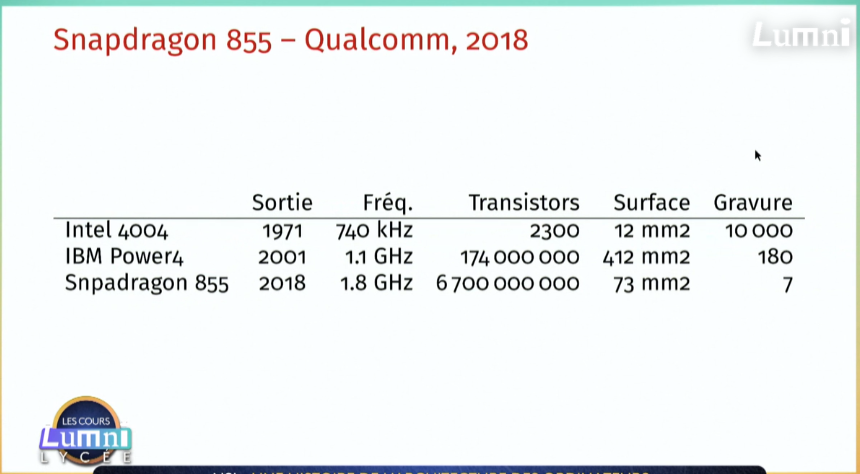
\includegraphics[scale=0.3]{images/miniaturisation.png}
\end{center}

\end{exercice}

\section{Architecture de Von Neumann}

\subsection{Un processeur pour calculer et une mémoire pour stocker programme et données}


\begin{cours}{}

Un ordinateur est une machine \textbf{programmable}, \textbf{automatique} et \textbf{universelle} :

\begin{itemize}
	
	\item \textbf{programmable} : la séquence d'opérations exécutée par un ordinateur peut être entièrement spécifiée dans le texte d'un programme ;
	\item \textbf{automatique} : un ordinateur peut exécuter un programme sans intervention extérieure (câblage \ldots) ;
	\item \textbf{universelle} : un ordinateur peut exécuter tout programme calculable (selon la théorie de Turing) avec le jeu d'instructions câblé dans son processeur.	

\end{itemize}

En 1945,  \href{https://fr.wikipedia.org/wiki/John_von_Neumann}{John von Neumann}, mathématicien hongrois exilé aux États-Unis, publie un rapport sur la réalisation du calculateur EDVAC où il propose une architecture permettant d'implémenter une machine universelle, décrite par \href{https://interstices.info/alan-turing-itineraire-dun-precurseur/}{Alan Turing} dans son article fondateur de 1936 sur le problème de l'indécidabilité. 

L'\textbf{architecture de Von Neumann }va servir de modèle pour la plupart des ordinateurs de 1945 jusqu'à nos jours, elle se compose de quatre parties distinctes :

\begin{itemize}[label=\ding{43}]

\item Le \textbf{CPU} (\textit{Central Processing Unit}), ou \textbf{processeur }constitué de :
	\begin{itemize}
		\item L'\textbf{Unité Arithmétique et Logique} (ALU en anglais) qui réalise des opérations arithmétiques (addition, multiplication \ldots), logiques (et, ou \ldots), de comparaisons ou de déplacement de mémoire (copie de ou vers la mémoire). L'ALU stocke les données dans des mémoires d'accès très rapide appelées \textbf{registres}. Les opérations sont réalisées par des circuits logiques constituant le \textbf{jeu d'instructions} du processeur. 
	   \item L'\textbf{Unité de Contrôle} charge la prochaine instruction dont l'adresse mémoire se trouve dans un registre appelé \textbf{Compteur de Programme} (PC en anglais), la décode et commande l'exécution par l'ALU. L'instruction en cours d'exécution est chargée dans le \textbf{Registre d'Instruction}. L'\textbf{Unité de Contrôle} peut aussi effectuer une opération de branchement, un saut dans le programme, en modifiant le \textbf{Compteur de Programme}, qui par défaut est incrémenté de $1$ lors de chaque instruction.
	\end{itemize}
	
\item La \textbf{mémoire} où sont stockés les \textbf{données} et les \textbf{programmes}.
\item Des \textbf{bus} qui sont des fils reliant le \textbf{CPU} et la \textbf{mémoire} et permettant les echanges de données et d'adresses.
\item Des dispositifs d'\textbf{entrées/sorties} permettant d'échanger avec l'extérieur (lecture ou écriture de données).
\end{itemize}

\textbf{Dans le modèle de Von Neumann, le processeur exécute une instruction à la fois, de façon séquentielle.} 


\begin{center}
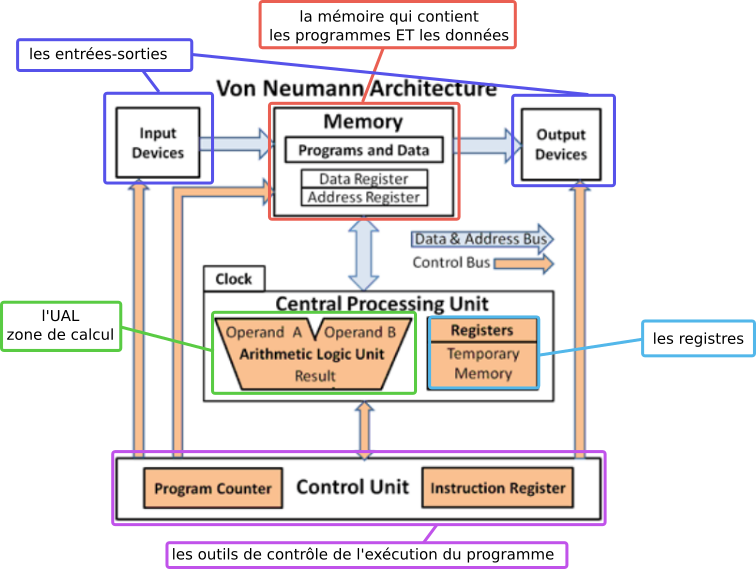
\includegraphics[scale=0.5]{images/arch.png}

{\itshape \uline{source :} Gilles Lassus }
\end{center} 

\end{cours}


\begin{courscomplement}{}

L'\textbf{Unité de Contrôle} réalise en boucle un cycle d'exécution rythmé par une horloge à quartz :

\begin{itemize}
	\item \textbf{Chargement}  de l'instruction pointée par le \textbf{Compteur de Programme} dans le \textbf{Registre d'Instruction}.
	\item \textbf{Décodage} de l'instruction stockée dans le \textbf{Registre d'Instruction} et chargement des opérandes.
	\item \textbf{Exécution} de l'instruction par \textbf{l'ALU} s'il s'agit d'une opération arithmétique ou logique ou par \textbf{l'Unité de Contrôle} s'il s'agit d'un branchement avec modification du \textbf{Compteur de Programme}.

\end{itemize} 

 Par exemple si l'horloge a une fréquence de $2,5$ gigahertz, $2,5$ milliards de cycles d'exécutions sont effectués par seconde.  Jusqu'en $\np{2004}$, la fréquence des processeurs a augmenté linéairement, mais depuis elle stagne à cause des problèmes de dissipation thermique. Les performances des ordinateurs sont améliorées par d'autres techniques (pipe-line,exécution en parallèle sur plusieurs coeurs de processeurs \ldots)

%Le \textbf{pipe-line d'instructions} est une évolution du modèle de Von Neumann, qui découpe  chaque instruction en étapes élémentaires confiées à des circuits indépendants. Par exemple, dans un pipe-line à cinq étages, une instruction se décompose en cinq étapes : FETCH (lecture), DEC (décodage), EXEC (exécution); MEM (accès mémoire) et RES (livraison du résultat). Le processeur peut exécuter en parallèle jusqu'à cinq instructions lorsque les circuits sont libérés. Ainsi l'exécution de cinq instructions ne nécessite plus que 9 cycles au lieu de 25.
%
%\begin{center}
%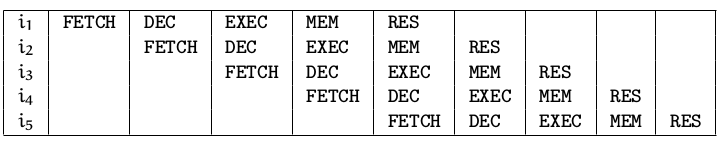
\includegraphics[scale=0.5]{images/pipeline.png}
%
%{\itshape \uline{source :}  Laurent Bloch }
%\end{center} 


\end{courscomplement}

\vspace*{-20pt}

\begin{exercice}{QCM type E3C}

\begin{enumerate}

\item Dans l'architecture générale de Von Neumann, la partie qui a pour rôle
d'effectuer les opérations de base est : 

\begin{tasks}[style=multiplechoice-alph](1)
\task  l'unité de contrôle
\task la mémoire
\task l'unité arithmétique et logique
\task les dispositifs d\'entrée-sortie
\end{tasks}

\item Parmi tous les registres internes que possède une architecture
mono-processeur, il en existe un appelé compteur ordinal \textit{program
counter}.

Quel est le rôle de ce registre ?


\begin{tasks}[style=multiplechoice-alph](1)
\task  il contient l'adresse mémoire de la prochaine instruction à exécuter
\task il contient le nombre d'instructions contenues dans le programme
\task il contient l'adresse mémoire de l'opérande à récupérer
\task il contient le nombre d'opérandes utilisés
\end{tasks}


\end{enumerate}



\end{exercice}

\subsection{Hiérarchie des mémoires}






\begin{cours}{}

On distingue plusieurs types de mémoires suivant leur \textbf{persistance}, leur \textbf{capacité}, leur \textbf{rapidité d'accès}.  Tous les types de mémoire utilisent une unité élémentaire d'information qui peut prendre deux états $0$ ou $1$ qu'on appelle \textbf{binary digit} ou \textbf{bit}.

\begin{itemize}[label=\ding{43}]

	\item Une \textbf{mémoire vive} ou \textbf{volatile} nécessite une alimentation électrique, elle est non persistante mais d'un accès rapide :
	
	\begin{itemize}
		\item Un \textbf{registre} est une mémoire de très petite capacité mais d'accès rapide car elle est  située directement dans le processeur.
		\item La \textbf{mémoire centrale}, ou \textbf{Random Access Memory} est une mémoire de grande capacité. 
		
		
Les bits disponibles sont regroupés par blocs en \textbf{mots mémoires} de même taille. Celle-ci correspond à la largeur d'un registre : $32$ bits ou $64$ bits actuellement. C'est aussi la taille de l'adresse repérant un mot mémoire. En pratique, on peut adresser des blocs de $8$ bits appelés \textbf{octets}.  Un processeur avec des registres de  $32$ bits ne peut adresser plus de $2^{32}$ octets soit environ $4$ gigaoctets.  Chaque mot mémoire est adressable directement à partir de son adresse, on parle de \textbf{mémoire à accès direct}. 
		
		Le temps d'accès à la mémoire centrale est entre 5 et 50 fois supérieur à celui d'un registre, cette différence de vitesse entre le processeur et la mémoire est le \textbf{goulot d'étranglement de l'architecture de Von Neumann}. 
		

		\item Pour améliorer les performances, une \textbf{mémoire cache}, placée entre le processeur et la \textbf{mémoire centrale} permet d'accéder plus rapidement aux instructions et données en cours d'utilisation qui ont une plus grande probabilité d'être réutilisées.
	\end{itemize}

   \item Une \textbf{mémoire persistante} ou \textbf{non volatile} permet de stocker des données sans alimentation électrique, avec d'autres procédés physiques (disques  magnétiques) : 
   
   \begin{itemize}
   	\item Les disques durs magnétiques ou SSD,  permettent de stocker  données et  programmes, dont le système d'exploitation, chef d'orchestre de tous les programmes. Leur capacité est presque $500$ fois supérieure à  celle de la mémoire centrale mais avec un temps d'accès inversement proportionnel.  Le \textbf{système d'exploitation} peut étendre virtuellement la mémoire centrale en utilisant les capacités des mémoires persistantes (\textbf{swapping})
   	\item La carte mère d'un ordinateur contient des données nécessaires au démarrage dans la \textbf{mémoire morte} ou \textbf{Read Only Memory}. Cette mémoire n'est pas modifiable.
   \end{itemize}
   
\end{itemize}

\begin{center}
\begin{tabular}{|c|c|c|c|}
\hline 
\textbf{mémoire} & \textbf{temps d'accès} & \textbf{débit} & \textbf{capacité} \\ 
\hline 
registre & 1 ns &  & $\approx$ Kio \\ 
\hline 
 mémoire cache & $2-3$ ns &  & $\approx$ Mio \\ 
\hline 
RAM & $5-60$ ns & $1-20$ Gio/s & $\approx$ Gio \\ 
\hline 
disque dur & $3-20$ ms & $10-320$ Mio/s & $\approx$ Tio \\ 
\hline 
\end{tabular} 
\end{center}


\textbf{Lorsqu'on se rapproche du processeur,  le coût de la mémoire et sa rapidité d'accès augmentent tandis que sa  capacité diminue.}


\begin{center}
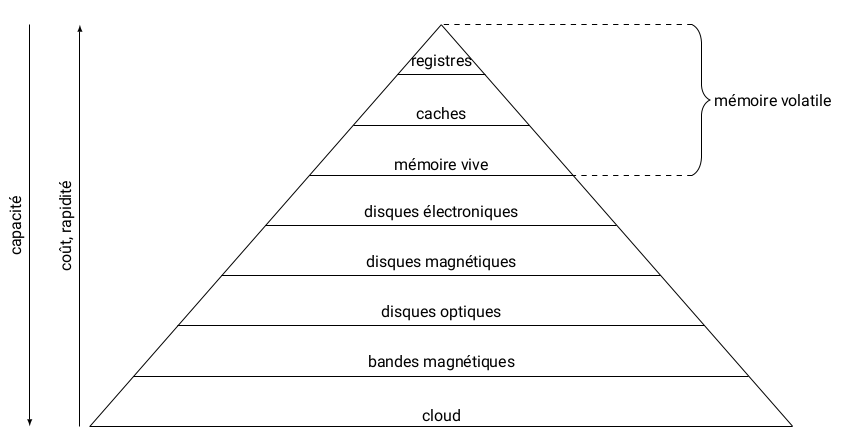
\includegraphics[scale=0.5]{images/hierarchie_memoire.png}
\end{center}

\end{cours}


\begin{exercice}{}

Pour mesurer une quantité d'information en informatique, on utilise l'octet représentant $8$ bits.

Les préfixes multiplicateurs les plus utilisés sont définis en base 10 : 1 kilooctet (Ko) $\,=\, 10^{3}$ octets, 1 mégaoctet (Mo)  $\,=\,10^{6}$ octets, 1 gigaoctet (Go)  $\,=\,10^{9}$ octets.

Il existe aussi des préfixes multiplicateurs en base 2  :  1 kibioctet (Kio) $\,=\, 2^{10}\,=\, \np{1024}$ octets, 1 mébioctet (Mio)  $\,=\, 2^{20}\,\approx\, \np{1,049}$ mégaoctet, 1 gibioctet (Gio)  $\,=\, 2^{30}\,\approx\, \np{1,074}$ gigaoctet.


\begin{enumerate}
	\item Quelle taille de mémoire centrale en octets peut-on adresser avec un processeur d'architecture $64$ bits ?
\item Un disque dur a une capacité de 500 Go. Exprimer cette capacité en Gio.
\item Sachant qu'une minute de musique au format mp3 occupe un espace de 1 Mo, combien d'heures de musique peut-on stocker sur un baladeur de 18 Go.
\item Avec un débit de 80 Mbits/s, combien de temps faut-il pour télécharger un fichier de 1,8 Go ?
\end{enumerate}

\end{exercice}

\section{Langage machine et assembleur}


\subsection{Du texte d'un langage de programmation aux instructions du langage machine}

\begin{cours}{}

Les programmes stockés dans la mémoire centrale de l'ordinateur sont constitués d'instructions de bas niveau, exécutables directement par les circuits logiques du processeur. Le \textbf{jeu d'instructions} du microprocesseur est restreint.  L'unité de contrôle décode la série de bits composant chaque instruction : les premiers bits forment un code (\textbf{opcode}) qui déclenche l'activation des circuits nécessaires dans l'ALU et les bits suivants portent les opérandes. 

Un programme nommé \textbf{compilateur} permet de transformer le texte d'un programme en langage de haut niveau (comme \texttt{Python} ou \texttt{C}) en une série d'instructions en langage machine.

\texttt{Python} est un langage permettant une exécution en direct dans un interpréteur sans production de fichier binaire comme en \texttt{C}. L'opération de compilation se passe différemment : lors de l'exécution d'un code \texttt{Python}, le texte du programme est d'abord compilé en \texttt{bytecode} qui est ensuite exécuté par une machine virtuelle (l'interpréteur). \texttt{Python} peut ainsi être exécuté sur n'importe quel processeur, alors que pour un langage compilé comme \texttt{C}, il faut un compilateur adapté au processeur pour produite l'exécutable binaire à partir d'un programme source.

Un \textbf{langage d'assembleur} est un intermédiaire lisible par un humain, entre le langage machine et un langage de haut niveau. Il traduit les instructions du langage machine par des \textbf{symboles} ou \textbf{mnémoniques}. Il est possible d'écrire  un programme en assembleur (dépendant du processeur) et un programme nommé également assembleur, le traduira directement en langage machine.

\begin{center}
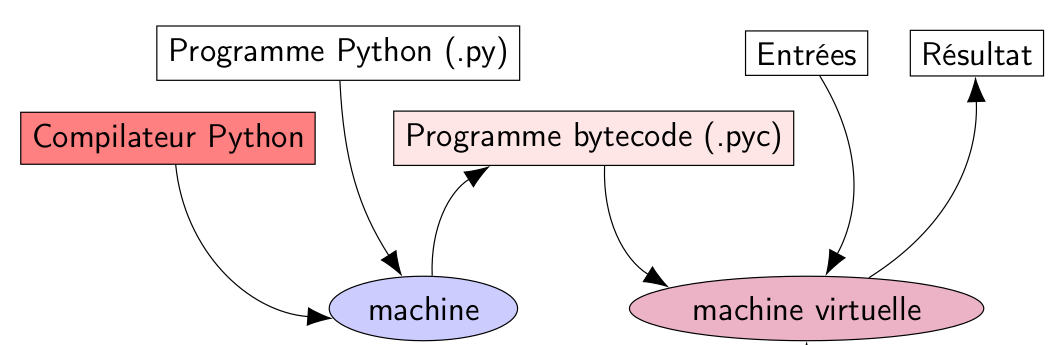
\includegraphics[scale=0.4]{images/python_bytecode.png}

{\itshape \uline{source :} Judicael Courant }
\end{center}


\end{cours}


\begin{exercice}{}

On peut récupérer tous les fichiers nécessaires pour cet exercice dans l'archive \href{}{compilation.zip}.

On donne ci-dessous le texte d'un programme \texttt{exemple.c} écrit  en langage \texttt{C}.

\begin{lstlisting}[language=C,numbers=left]
#include "stdlib.h"

int main()
{
int a = 5;
a =  a + 3;
return 0;
} 
\end{lstlisting}

\begin{enumerate}

\item 

\begin{enumerate}
	\item Récupérer le fichier source du programme \texttt{exemple.c}.
	\item Compiler le programme pour produite le fichier binaire \texttt{exemple} avec la commande \texttt{gcc exemple.c -o exemple}.
	
Rendre exécutable le binaire avec la commande \texttt{chmod +x exemple} puis l'exécuter avec \texttt{exemple} et constater avec \verb+echo $?+ que le programme s'est exécuté sans erreur (sortie $0$).

\begin{lstlisting}[style=compil]
fred@portable:~/sandbox$ gcc exemple.c -o  exemple
fred@portable:~/sandbox$ chmod +x exemple
fred@portable:~/sandbox$ ./exemple 
fred@portable:~/sandbox$ echo $?
0
\end{lstlisting}

	\item Si on édite le fichier \texttt{exemple} avec un éditeur de textes, obtient-on un affichage lisible ?
	\item Afficher le contenu du fichier binaire \texttt{exemple} avec un éditeur hexadécimal en ligne comme \url{https://hexed.it/}.
	
	\item Récupérer dans un fichier texte le code d'assembleur généré à partir du  fichier source \texttt{exemple.c} avec la commande :

\begin{lstlisting}[style=compil]
fred@portable:~/sandbox$ gcc exemple.c  -o - -S > assembleur.txt
\end{lstlisting}

\item On donne ci-dessous le texte du programme en assembleur x86. 

\verb+%eax+ désigne les quatre premiers octets du registre accumulateur, recevant les résultats des calculs , tandis que \verb+%rsp+ et \verb+%rbp+  sont des registres pointant respectivement vers la base et le sommet de la pile, une zone de la mémoire centrale dédiée au programme.  De plus \verb+-4(%rbp)+ désigne une adresse mémoire située 4 octets en-dessous de  la base de la pile.

À partir du guide fourni sur \url{http://www.lsv.fr/~goubault/CoursProgrammation/Doc/minic007.html}, expliquer les instructions des lignes 13, 14 et 15.


\begin{lstlisting}[numbers=left, language={[x86masm]Assembler}]
	.file	"exemple.c"
	.text
	.globl	main
	.type	main, @function
main:
.LFB2:
	.cfi_startproc
	pushq	%rbp
	.cfi_def_cfa_offset 16
	.cfi_offset 6, -16
	movq	%rsp, %rbp
	.cfi_def_cfa_register 6
	movl	$5, -4(%rbp)
	addl	$3, -4(%rbp)
	movl	$0, %eax
	popq	%rbp
	.cfi_def_cfa 7, 8
	ret
	.cfi_endproc
.LFE2:
	.size	main, .-main
	.ident	"GCC:(Ubuntu 5.4.0-6ubuntu1~16.04.12) 5.4.0 20160609"
	.section	.note.GNU-stack,"",@progbits
\end{lstlisting}

\end{enumerate}

\item 




Le module \texttt{dis} de la bibliothèque standard  permet de désassembler le \texttt{bytecode} produit par un code source \texttt{Python} pour obtenir les instructions du compilateur \texttt{Python} ayant permis de le générer.

\begin{enumerate}
\item Créer un nouveau fichier ou notebook \texttt{Python} puis saisir le programme ci-dessous :

\begin{lstlisting}[style=rond]
import dis 

code_source = """
a = 5
a = a + 3
"""

dis.dis(code_source)
\end{lstlisting}

À partir de la documentation \url{https://docs.python.org/3/library/dis.html}, expliquer la traduction du programme contenu dans \verb+code_source+ en assembleur \texttt{Python}. Comparer avec la traduction d'un programme similaire obtenue précédemment  en assembleur \texttt{x86}.

\begin{lstlisting}[style=compil]
2           0 LOAD_CONST               0 (5)
              3 STORE_NAME               0 (a)


3           6 LOAD_NAME                0 (a)
              9 LOAD_CONST               1 (3)
             12 BINARY_ADD
             13 STORE_NAME               0 (a)
             16 LOAD_CONST               2 (None)
             19 RETURN_VALUE
\end{lstlisting}

\item Afficher les codes numériques des instructions du programme contenu dans \verb+code_source+ en  assembleur \texttt{Python} avec le programme ci-dessous.

\begin{lstlisting}[style=rond]
print(list(dis.get_instructions(code_source)))

code = compile(code_source, '<string>','exec')
for octet in code.co_code:
    print(octet, end = ' ')
\end{lstlisting}

\end{enumerate}

\end{enumerate}
\end{exercice}





\subsection{Premiers programmes en assembleur avec le simulateur Aqua}

\begin{methode}{}

Nous allons utiliser un simulateur d'architecture de Von Neumann, réalisé par Peter Higginson pour préparer des étudiants anglais à leur examen de Computer Science. Il se nomme AQUA et on peut l'exécuter en ligne sur  \url{http://www.peterhigginson.co.uk/AQA/}. 

Quelques principes de base :

\begin{itemize}
\item On ne peut pas définir de variables. Les données manipulées sont soient stockées à un endroit précis en mémoire soit dans un des registres R0 à R12. 

\item Il n'existe pas de structure de contrôle conditionnelle comme le "if \ldots then \ldots  else" ou les boucles "while", "for". Pour les implémenter, on utilise des instructions de saut inconditionnel ou conditionnel en fonction du résultat de la comparaison précédente. Les points de chute de saut sont repérés par des étiquettes placées dans le programme.

\item Pour calculer avec une donnée en mémoire, il faut d'abord la transférer dans un registre.

\end{itemize}

L'interface se divise verticalement en trois zones :

	\begin{itemize}
	
		\item À gauche, l'éditeur de programme en assembleur. On remplit le formulaire et on le soumet avec \texttt{submit}, puis on assemble le programme en mémoire avec \texttt{assemble} et on l'exécute avec \texttt{run}. Plusieurs vitesses d'exécution sont disponibles.
		
		\item Au centre, le \textbf{processeur}, avec les treize registres de données de R0 à R12, le \textbf{Compteur de Programme PC}, l' \textbf{Unité de Contrôle} avec son \textbf{Registre d'Instruction CIR} et l'\textbf{ALU} avec ses quatre drapeaux de test (Z pour zéro, N pour négatif, C pour carry, retenue et V pour overflow). Les bus reliant les différents composants du processeur et la mémoire sont en bleu. Les registres MAR et MBR servent à transférer des données entre la mémoire et les registres : MAR contient l'adresse (en décimal) où l'on veut lire ou écrire et MBR la valeur lue ou à écrire (en hexadécimal). 
		
		\item À droite, la mémoire divisée en mots de largeur $32$ bits et dont les adresses commencent  à $0$. Dans \texttt{options} on peut choisir le format d'affichage (décimal signé ou non, binaire, hexadécimal).
	\end{itemize}	


\begin{center}
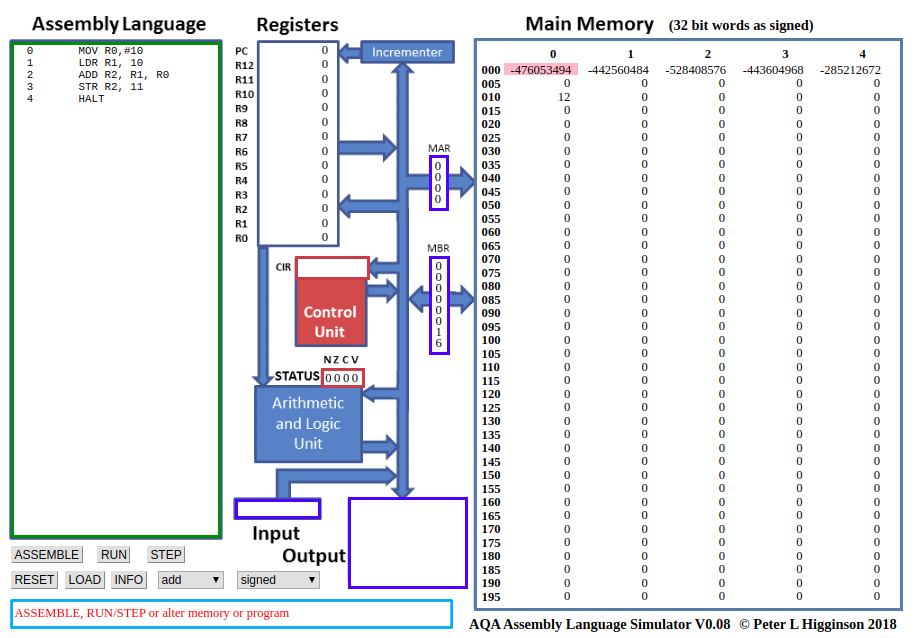
\includegraphics[scale=0.55]{images/simulateur_aqua.png}
\end{center}

Le jeu d'instructions est précisé dans la documentation \url{http://peterhigginson.co.uk/AQA/info.html}.

Voici quelques exemples d'instructions d'opérations arithmétiques et de transfert de mémoire :

\begin{center}
\begin{tabular}{|p{0.2\linewidth}|p{0.75\linewidth}|}
\hline 
\textbf{Instruction} & \textbf{Traduction} \\ 
\hline 
\texttt{LDR R1,78} & Charge dans le registre R1 la valeur stockée en mémoire à l'adresse $78$ \\ 
\hline 
\texttt{STR R1,123} & Stocke le contenu du registre R1 à l'adresse $123$ en mémoire \\ 
\hline
\texttt{LDR R1,[R2]} & Charge dans le registre R1 la valeur stockée en mémoire à l'adresse contenue dans le registre R2 \\ 
\hline 
\texttt{ADD R1,R0,\#128} & Additionne le nombre 128 (une valeur immédiate est identifiée grâce au symbole \#) et la valeur stockée dans le registre R0, place
le résultat dans le registre R1 \\ 
\hline 
\texttt{SUB R1,R0,\#128} & Soustrait le nombre 128 de la valeur stockée dans le registre R0, place le résultat dans le registre R1 \\ 
\hline 
\texttt{SUB R0,R1,R2} & Soustrait la valeur stockée dans le registre R2 de la valeur stockée dans le registre R1, place le résultat dans le registre R0 \\ 
\hline 
\texttt{MOV R1,\#23} & Place le nombre 23 dans le registre R1 \\ 
\hline 
\texttt{MOV R0, R3} & Place la valeur stockée dans le registre R3 dans le registre R0 \\ 
\hline 
\texttt{HALT} & Symbole de fin de programme, indispensable pour que le programme se termine sans erreur \\ 
\hline
\end{tabular} 
\end{center}


\end{methode}


\begin{exercice}{}


\begin{enumerate}
	\item Ouvrir le simulateur AQUA depuis le lien sur le bureau ou le Web : \url{http://www.peterhigginson.co.uk/AQA/}.
	
	\item Saisir le programme ci-dessous dans la fenêtre d'édition puis le soumettre avec \texttt{submit}.
	
\begin{lstlisting}[numbers=left]
MOV R0, #10
LDR R1, 10
ADD R2, R1, R0
STR R2, 11
HALT
\end{lstlisting}

\item Assembler le programme avec \texttt{assemble} et modifier le mot mémoire d'adresse $10$ en lui donnant la valeur $12$. Sélectionner ensuite l'affichage binaire.

\item A quoi correspond le mot de $32$ bits contenu en mémoire à l'adresse $0$ : \texttt{11100011 10100000 00000000 00001010} ?

\item  Repérer les  mots mémoires de $32$ bits stockant le programme et le mot mémoire stockant la donnée $12$.

\item Sélectionner l'affichage \texttt{Unsigned}. Exécuter le programme pas à pas (\texttt{step})  en vitesse lente (\texttt{options} puis \texttt{def slow}).

Décrire l'enchaînement d'opérations élémentaires lors de l'exécution des instructions de transfert de mémoire \texttt{MOV R0,\#10} puis \texttt{LDR R1,10}. Observer l'évolution des registres PC (Compteur de programme), CIR (Registre d'instructions), MAR (adresse d'écriture/lecture en mémoire) et MBR (donnée à lire/écrire). Pour quelle(s) instruction(s), l'\textbf{ALU} est-elle sollicitée ?
     



\end{enumerate}

\end{exercice}


\begin{exercice}{}

On considère le programme en assembleur ci-dessous. 

Les commentaires sont précédés des caractères \verb+//+.

\begin{enumerate}
	\item Décrire la modification de l'état de la mémoire (registre et mémoire centrale) provoquée par la séquence  d'instruction d'\textit{initialisation} des lignes $2$ à $6$.
	  \item Décrire la modification de l'état de la mémoire (registre et mémoire centrale) provoquée par la séquence  d'instruction de \textit{l'itération 1} des lignes $8$ à $11$.
	  \item Où sont stockées dans la mémoire centrale les quatre valeurs calculées par ce programme ? Il s'agit des premières valeurs d'une suite célèbre, laquelle ? Quelle structure algorithmique serait nécessaire pour calculer les termes suivants sans copier-coller ?
	  \item Rajouter les calculs de deux termes supplémentaires de la suite, par copier-coller des lignes $23$ à $26$, puis exécuter le programme dans le simulateur. Observer l'état de la mémoire, expliquer  l'erreur signalée  par l'Unité de Contrôle et corriger le programme.
\end{enumerate}

\begin{lstlisting}[numbers=left, language={[x86masm]Assembler}]
//initialisation
MOV R0, #25
MOV R1, #1
STR R1, [R0]
ADD R0, R0, #1
MOV R2, #1
//itération 1
STR R2, [R0]
ADD R2, R2, R1
LDR R1, [R0]
ADD R0, R0, #1
//itération 2
STR R2, [R0]
ADD R2, R2, R1
LDR R1, [R0]
ADD R0, R0, #1
//itération 3
STR R2, [R0]
ADD R2, R2, R1
LDR R1, [R0]
ADD R0, R0, #1
//itération 4
STR R2, [R0]
ADD R2, R2, R1
LDR R1, [R0]
ADD R0, R0, #1
//fin
HALT
\end{lstlisting}

\end{exercice}


\begin{exercice}{}


On considère le programme \texttt{Python} ci-dessous
\begin{lstlisting}[style=rond]
a = 42      #valeur 42 à l'adresse 20 en mémoire centrale
b = 69      #valeur 69 à l'adresse 21 en mémoire centrale
a = a + b   #changement de valeur à l'adresse 20
b = a - b   #changement de valeur à l'adresse 21
a = a - b   #changement de valeur à l'adresse 20
\end{lstlisting}

\begin{enumerate}
	\item Déterminer le contenu des variables \texttt{a} et \texttt{b} à la fin de l'exécution de ce programme \texttt{Python}.
	\item Traduire ce programme en assembleur et le tester dans le simulateur.

\bcattention{} En assembleur, les identifiants de variables sont remplacés par des adresses en mémoire centrale et les opérations arithmétiques ne sont effectuées que sur des registres, il faut donc d'abord transférer les opérandes de la mémoire centrale vers des registres.

\end{enumerate}


\end{exercice}


\subsection{Programmer une instruction conditionnelle en assembleur}


\begin{methode}{}

Dans le programme assembleur ci-dessous, on introduit de nouveaux symboles :

\begin{itemize}[label=\ding{43}]
	\item \texttt{INP R1,2} est une \textbf{instruction d'entrée}, qui lit un entier  saisi dans le champ Input et le charge dans le registre \texttt{R1}.
	\item \texttt{OUT R1,4} est une \textbf{instruction de sortie}, qui affiche le contenu du registre \texttt{R1} dans le champ Output.
	\item \texttt{else:} et \texttt{fin:} sont des \textbf{étiquettes} qui jouent le rôle de repères / points de chute,  dans les instructions de branchement / saut. Une étiquette est un mot suivi du symbole colonne \texttt{:}
	\item \texttt{CMP R0,\#0} est une instruction de comparaison qui compare le contenu du registre \texttt{R0} au nombre $0$.   Elle est suivie d'une instruction de \textbf{branchement (ou saut) conditionnel}   \texttt{BLT else} : le programme se poursuit soit à partir de l'étiquette \texttt{else} si \texttt{R0} est plus petit que $0$, sinon  avec l'instruction de la ligne suivante (comportement par défaut).
	\item  \texttt{B fin} est une instruction de \textbf{branchement / saut inconditionnel} : le programme se poursuit  à partir de l'étiquette \texttt{fin}, le flux normal (passage à la ligne suivante) est interrompu.
	

\end{itemize}


Pour bien comprendre, le fonctionnement des instructions de branchement, exécuter le programme dans le simulateur en mode pas à pas, avec une vitesse lente au niveau des instructions \texttt{BLT else} et \texttt{B fin}.  Effectuer un test avec une valeur positive $4$ et l'autre avec une valeur négative $-4$.

Noter que le \textbf{Compteur de Programme PC} est incrémenté par défaut  de $1$ pour chaque instruction mais qu'il peut être de plus modifié par une instruction de branchement.


\begin{lstlisting}[numbers=left, language={[x86masm]Assembler}]
//Lecture d'un entier dans Input et chargement dans le registre R0
      INP R0, 2
//Comparaison du registre R0 avec le nombre 0
      CMP R0, #0
//Branchement conditionnel sur l'étiquette else si R0 négatif
      BLT else
      MOV R1, R0
//Branchement inconditionnel sur l'étiquette fin
      B fin
//étiquette else
else:
      MOV R2, #0
      SUB R1, R2, R0
//étiquette fin
fin:
//affichage du registre R1 dans Output
      OUT R1, 4
      HALT 
\end{lstlisting}



\end{methode}


\begin{exercice}{}


On considère le programme \texttt{Python} ci-dessous
\begin{lstlisting}[style=rond]
a = int(input())  #entier lu stocké dans le registre R0
b = int(input())  #entier lu stocké dans le registre R1
if a > b:
	m = a         
else:
	m = b
#le maximum m de a et b est stocké dans le registre R2
#et en mémoire centrale à l'adresse 20
print(m)
\end{lstlisting}

Traduire ce programme en assembleur puis le tester dans le simulateur.

\end{exercice}

\subsection{Programmer une boucle en assembleur}

\begin{methode}{}

Dans le simulateur AQUA, sélectionner puis exécuter le programme \texttt{ascii} en mode pas à pas. Observer l'évolution du \textbf{Compteur de Programme PC} lors de chaque exécution du branchement conditionnel \texttt{BLT LOOP}.

\begin{lstlisting}[numbers=left, language={[x86masm]Assembler}]
	  //initialise le registre R2 avec le nombre 32
      MOV R2,#32
LOOP:
	  //affiche dans Output le caractère dont le code ascii est contenu dans R2
      OUT R2,7
      //incrémente R2
      ADD R2,R2,#1
      //compare R2 avec 127
      CMP R2,#127
      //si R2 < 127 branchement conditionnel sur l'étiquette loop
      BLT LOOP
      //sinon le programme se poursuit
      MOV R2,#10
      //affichage du caractère de code ascii 10 qui est un saut de ligne
      OUT R2,7
      HALT
\end{lstlisting}

Ce programme permet d'afficher tous les caractères dont le code ascii est compris entre $32$ et $126$, par ordre croissant du code. C'est une implémentation de boucle \texttt{while} en assembleur, une traduction en \texttt{Python} pourrait être :

\begin{lstlisting}[style=rond]
code_ascii = 32
while code_ascii < 127:
    print(chr(code_ascii), end ='')
    code_ascii = code_ascii + 1
print()
\end{lstlisting}

\end{methode}


\begin{exercice}{}

\begin{enumerate}
	\item Modifier le programme \texttt{ascii} pour qu'il affiche tous les caractères dont le code ascii est compris entre $126$ et $32$ dans l'ordre décroissant du code.
	
	\item Modifier le programme de l'exercice 7, pour qu'il stocke en mémoire à partir de l'adresse $20$, les $30$ premiers termes de cette suite célèbre.
	
	\item Traduire en assembleur le programme \texttt{Python} ci-dessous. On peut utiliser uniquement des registres.
	
\begin{lstlisting}[style=rond]
s = 0
k = 1
while k <= 100:
	s = s + k
	k = k + 1
print(s)
\end{lstlisting}

	\item Traduire en assembleur le programme \texttt{Python} ci-dessous. On peut utiliser uniquement des registres.

\bcattention{} Le langage d'assembleur du simulateur AQUA ne dispose pas d'instruction pour multiplier deux nombres.

 
\begin{lstlisting}[style=rond]s = 0
a = int(input())
b = int(input())
c = a * b
print(c)
\end{lstlisting}


\item Traduire en assembleur le programme \texttt{Python} ci-dessous. On peut utiliser uniquement des registres.

\begin{lstlisting}[style=rond]s = 0
code_ascii = 32
while code_ascii < 127:
	i = 0
	while i < 10:
		#affichage du caractère sans saut de ligne
		print(chr(code_ascii), end ='') 
    code_ascii = code_ascii + 1
	print()    #saut de ligne
\end{lstlisting}

\end{enumerate}

\end{exercice}


\begin{center}
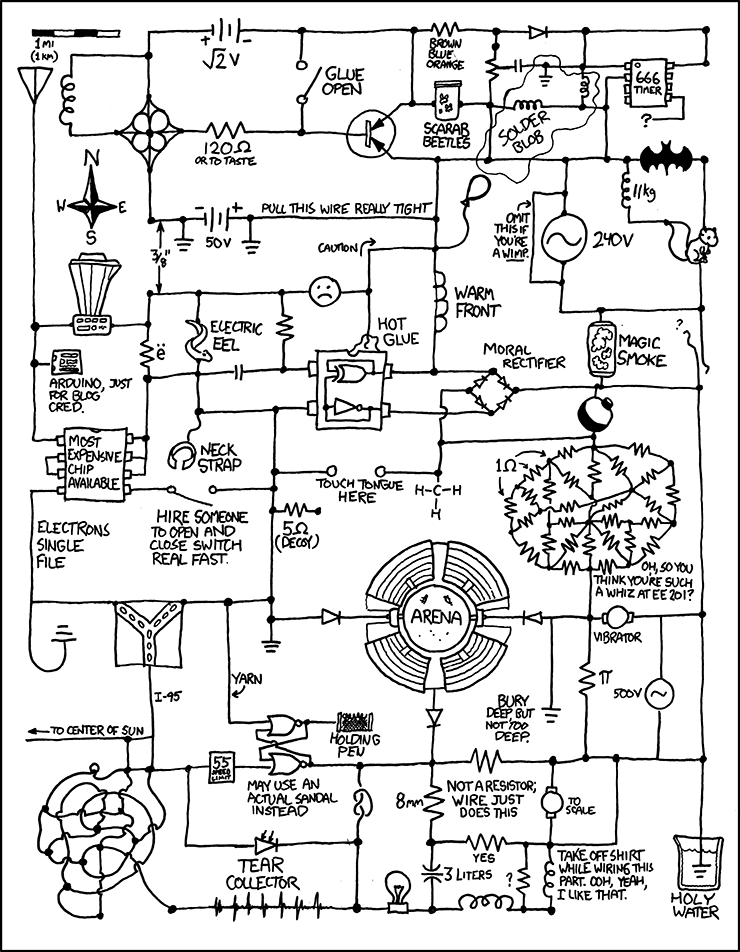
\includegraphics[scale=0.35]{images/circuit_diagram.png}

\url{https://xkcd.com/730/}
\end{center}



 \end{document}
